\documentclass[openany]{fast-nuces-bs}
\usepackage{mathptmx}
\usepackage[T1]{fontenc}
\usepackage{sectsty}
\usepackage{tikz-uml}
\usepackage{titlesec}
\usepackage{graphicx}
\usepackage[table]{xcolor}
\usepackage{booktabs}
\usepackage{longtable}
\usepackage{tabularx}
\usepackage{array}
\usepackage{ragged2e}
\usepackage{enumitem}
\usepackage{float}
\usepackage{microtype}
\usepackage{url}
\usepackage{setspace}
\usepackage{needspace}
\usepackage{etoolbox}

\department{FAST School of Computing}
\faculty{Computer Science}
\degreeyear{2026}
\degreemonth{December}
\degreename{Computer Science}
\campuscity{Islamabad}
\authorone{Shahmeer Amir}{23I-0626}
\authortwo{Faizan ur Rehman Khan}{23I-3021}
\authorthree{Ali Sher}{23I-0683}
\supervisor{Ms. Marium Hida}
\sessionduration{2023-2027}
\deanname{Dr. Dean Computing}
\directorname{Dr. Director of the Campus}
\hodname{Dr. Head of Computer Science Department}
\fypcoordinatorname{Name of FYP Coordinator}
\title{Aegis: A Spatio-Temporal Memory System for Assistive Care}

\onehalfspacing
\setlength{\parindent}{0pt}
\setlength{\parskip}{6pt plus 1pt}
\renewcommand{\arraystretch}{1.2}
\setlist{itemsep=3pt,topsep=2pt,parsep=0pt}
\setlist[itemize]{leftmargin=*}
\newcolumntype{Y}{>{\RaggedRight\arraybackslash}X}
\newcolumntype{L}[1]{>{\RaggedRight\arraybackslash}p{#1}}
\newcommand{\frontchapter}[1]{\chapter*{#1}\addcontentsline{toc}{chapter}{#1}\markboth{#1}{}}
\newcommand{\aegisfig}[4][\textwidth]{%
  \needspace{0.58\textheight}%
  \begin{figure}[H]\centering
  \IfFileExists{ThesisFigs/#2.png}{\includegraphics[width=#1,height=0.55\textheight,keepaspectratio]{ThesisFigs/#2.png}}{\fbox{\parbox[c][5cm][c]{0.85\textwidth}{\centering Missing figure: ThesisFigs/#2.png}}}
  \caption{#3}\label{#4}\end{figure}}
% Tall slot for figures that need most of a page (DIAGRAM_SPECS.md §0.4).
\newcommand{\aegisfigtall}[4][\textwidth]{%
  \needspace{0.88\textheight}%
  \begin{figure}[H]\centering
  \IfFileExists{ThesisFigs/#2.png}{\includegraphics[width=#1,height=0.85\textheight,keepaspectratio]{ThesisFigs/#2.png}}{\fbox{\parbox[c][5cm][c]{0.85\textwidth}{\centering Missing figure: ThesisFigs/#2.png}}}
  \caption{#3}\label{#4}\end{figure}}
% Red marks every item the team must still supply or confirm.
\newcommand{\tbd}[1]{\textcolor{red}{#1}}
% allow line breaks in long code identifiers (after _ and /) and loosen spacing
\let\aegisus\textunderscore
\DeclareRobustCommand{\_}{\aegisus\penalty50\hskip0pt\relax}
\setlength{\emergencystretch}{3em}
\newcommand{\captionof}[2]{\refstepcounter{#1}\addcontentsline{lot}{table}{#2}\textbf{Table \thetable. #2}\par}
\newcommand{\uctable}[8]{%
  \begin{singlespace}\small\captionof{table}{#1}\vspace{2pt}
  \noindent\begin{tabularx}{\textwidth}{@{}>{\bfseries}L{3cm}Y@{}}\toprule
  \rowcolor{gray!15}\textbf{Field}&\textbf{Description}\\\midrule
  Primary actor&#2\\ Preconditions&#3\\ Trigger&#4\\ Main flow&#5\\ Alternate flows&#6\\ Postconditions&#7\\ Related FRs&#8\\\bottomrule
  \end{tabularx}\end{singlespace}\par\vspace{8pt}}
\newenvironment{ltab}{\par\penalty0\relax\ifdim\dimexpr\pagegoal-\pagetotal\relax<12\baselineskip\relax\newpage\fi\small\setlength{\tabcolsep}{1pt}\setlength{\LTleft}{0pt}\setlength{\LTright}{0pt}\setlength{\LTcapwidth}{\textwidth}}{\par\vspace{0.5\baselineskip}}
\newcommand{\signatureblock}{%
  \par\vspace{1.2cm}\noindent
  \begin{tabularx}{\textwidth}{@{}L{6.4cm}Y@{}}
  \textbf{Shahmeer Amir} (23I-0626) & Signature: \hrulefill\\[1.1cm]
  \textbf{Faizan ur Rehman Khan} (23I-3021) & Signature: \hrulefill\\[1.1cm]
  \textbf{Ali Sher} (23I-0683) & Signature: \hrulefill\\
  \end{tabularx}}
\setlength{\headheight}{14pt}
% Keep headings with the visual/table material that immediately follows them.
\pretocmd{\section}{\par\nointerlineskip\hrule height0pt\relax\needspace{0.30\textheight}}{}{}
\pretocmd{\subsection}{\par\nointerlineskip\hrule height0pt\relax\needspace{0.40\textheight}}{}{}
\AtBeginEnvironment{table}{\needspace{0.30\textheight}}
\definecolor{ink}{HTML}{1F2933}
\definecolor{slate}{HTML}{52606D}
\definecolor{hdrfill}{HTML}{E4E7EB}
\definecolor{rowfill}{HTML}{F5F6F8}

\begin{document}
\cleardoublepage
\pagenumbering{roman}
\frontchapter{Students' Submission}
We certify that this report is submitted as the FYP-1 final report for the
project titled \textbf{Aegis: A Spatio-Temporal Memory System for Assistive Care}.
\signatureblock

\frontchapter{Anti-Plagiarism Statement}
The students certify that this report is their own work and that all sources
used in preparing the report have been appropriately acknowledged and
referenced.
\signatureblock

\frontchapter{Authors' Declaration}
We declare that the work documented in this report represents the work
completed by the project team up to the end of FYP-1. Contributions, tools,
external components and relevant sources are disclosed where applicable.
Generative-AI tools were used as coding and drafting aids; they are disclosed
per member in Section~\ref{sec:tools}, and all technical claims, designs and
results remain the responsibility of the team.
\signatureblock

\frontchapter{Abstract}
People with subjective cognitive decline, mild cognitive impairment, or
dementia often lose track of where they placed objects and whether they
completed daily tasks, which erodes independence and burdens caregivers. Among
the systems reviewed in this report, none combines a persistent, spatially
grounded memory of first-person experience with progressive temporal
compression and evidence-based natural-language querying for both the person
and a delegated caregiver. This report presents \textbf{Aegis}, an egocentric
spatio-temporal vision system that turns a wearable first-person video stream
into a multi-resolution memory of objects, layout, and activities: recent
history is kept in fine detail, older history is condensed into summaries.
Users and caregivers ask spatial and temporal questions by speech or text and
receive answers grounded in stored evidence, with an explicit ``not sure''
response when evidence is weak.

The project follows an iterative, vertical-slice approach. Iteration~1 (to the
mid-evaluation) delivered the batch reconstruction, perception and scene-graph
slice. Iteration~2 turned it into one end-to-end pipeline: live phone capture
with criterion-based keyframes, gap and pause records and crash-safe resume; a
gravity-aligned spatial model with nine object--anchor relations; debounced
object state runs; a persistent per-home SQLite memory with cross-session
matching of rooms, anchors and objects; verified three-day-then-summary
compaction; a rule-based, closed-vocabulary query engine served from Modal over
HTTPS; and patient and caregiver Flutter applications with on-device speech
input. The automated suite has 451 passing tests (79\% line coverage).
Component measurements show an open-vocabulary detection F1 of 0.721 on a
ten-frame, five-environment hand-labelled benchmark, and a 5.7--7.2$\times$
smaller memory with 100\% semantic retention on two short clips. A seven-day
public egocentric study (EgoLife) found that individual objects remained in
memory for one to four days, but class-level queries did not yet benefit from
the longer history. Temporal questions, calibrated confidence, caregiver
authentication, latency and usability remain unmeasured or planned for FYP-2.

\medskip\noindent\textbf{Keywords:} egocentric vision, spatio-temporal memory,
scene graph, natural-language querying, assistive technology, cognitive
impairment, memory abstraction, caregiver access.

\frontchapter{Acknowledgments}
The project team acknowledges the guidance and support received from the
project supervisor, Ms.\ Marium Hida, faculty members, and other contributors.
The team also thanks the open-source model and framework communities whose
software made this prototype possible, and the authors of VGGT-$\Omega$, SAM~2,
SAM~3, DINOv3 and the EgoLife dataset for making their models and data publicly
available.

\frontchapter{Executive Summary}
\textbf{Motivation.} Cognitive decline makes everyday recall unreliable:
people misplace objects, forget whether tasks were done, and then rely on
caregivers who often were not present. The loop of manual searching and
caregiver reconstruction (Figure~\ref{fig:recall-loop}) wastes time and effort
for both parties, and the population affected is growing as societies age.

\textbf{Project.} Aegis is an assistive ``external episodic memory''. A
wearable first-person camera observes the user's indoor environment; the system
builds a persistent spatio-temporal memory of objects, layout, and activities,
keeps recent history in fine detail, and condenses older history into
summaries. Natural-language questions (``Where are my keys?'') are answered by
speech or text, with supporting evidence, for the user and, through a separate
caregiver application, for a caregiver (consent-based access is planned). Four
modules, each with a named lead, implement the pipeline
(Section~\ref{sec:modules}).

\textbf{Research findings.} We reviewed three closely related systems --
MemPal, R4DSG, and DAAAM -- plus CrossSense and the wider egocentric-memory
literature (Chapter~\ref{chap:research}). They show that voice-based object
retrieval from a wearable camera is feasible for older adults, that
anchor-relative memory can be built from RGB-only wearable video, and that
hierarchical spatio-temporal memory supports long-horizon questions. Among the
systems reviewed, none combines these with progressive temporal abstraction and
delegated caregiver querying; this is the gap Aegis targets. Since the
mid-evaluation the team ran its own component experiments: a detector
comparison that replaced YOLOE with SAM~3, a memory-compaction audit, and a
seven-day EgoLife study that exposed cross-session room-identity instability
(Section~\ref{sec:experiments}, Chapter~\ref{chap:testing}).

\textbf{Requirements and plan.} Chapter~\ref{chap:requirements} specifies eight
top-level functional requirements with 44 sub-requirements (six added since the
mid report, \tbd{pending supervisor approval}), 16 non-functional requirements,
35 acceptance checks with their FYP-1 results, a traceability matrix and a
requirements change log. Chapter~\ref{chap:plan} records two completed
iterations against plan; Iterations~3 and~4 remain for FYP-2.

\textbf{Implementation and validation status.} Iteration~2 delivered live
capture, a gravity frame, nine spatial relations, state runs, a persistent home
store with cross-session matching, verified compaction, the NLQ engine and
\path{/ask} endpoint on Modal, and patient and caregiver apps
(Chapter~\ref{chap:iter2}). The suite has 451 passing tests at 79\% coverage.
Measured results are detection F1 0.721, compaction 5.7--7.2$\times$ with 100\%
semantic retention, one end-to-end run, and the EgoLife study. Accuracy on a
held-out clip, latency p95, room metrics and usability remain unmeasured.

\textbf{Risks and remaining work.} The three main risks are now: (1)
cross-session room identity, because room linking uses an absolute radius in
scale-free reconstruction units; (2) temporal and activity questions, which the
engine currently declines; and (3) the absence of authentication and
encryption. FYP-2 addresses these in Iterations~3 and~4
(Chapter~\ref{chap:fyp2}).

\frontchapter{List of Abbreviations}
\noindent
\begin{tabularx}{\textwidth}{@{}>{\bfseries}l Y@{}}
AC    & Acceptance Criterion\\
API   & Application Programming Interface\\
ASR   & Automatic Speech Recognition\\
CCP   & Complex Computing Problem\\
CI/CD & Continuous Integration / Continuous Deployment\\
CORS  & Cross-Origin Resource Sharing\\
DEI   & Diversity, Equity, and Inclusion\\
DFD   & Data Flow Diagram\\
ERD   & Entity--Relationship Diagram\\
FP    & False Positive\\
FR    & Functional Requirement\\
FYP   & Final Year Project\\
GPU   & Graphics Processing Unit\\
IoU   & Intersection over Union\\
LLM   & Large Language Model\\
MCI   & Mild Cognitive Impairment\\
MJPEG & Motion JPEG\\
NFR   & Non-Functional Requirement\\
NL    & Natural Language\\
NLQ   & Natural-Language Query\\
NMS   & Non-Maximum Suppression\\
OBB   & Oriented Bounding Box\\
R4DSG & Relative 4D Scene Graph\\
RANSAC & Random Sample Consensus\\
Re-ID & Re-identification\\
RGB-D & Colour image plus depth\\
SAM   & Segment Anything Model\\
SC    & Success Criterion\\
SCD   & Subjective Cognitive Decline\\
SG    & Scene Graph\\
STT   & Speech-to-Text\\
TC    & Technical Challenge\\
UC    & Use Case\\
UTC   & Coordinated Universal Time\\
VGGT  & Visual Geometry Grounded Transformer\\
VLM   & Vision--Language Model\\
WCAG  & Web Content Accessibility Guidelines\\
\end{tabularx}

\cleardoublepage
\pagenumbering{arabic}
\chapter{Introduction and Project Vision}
\label{chap:intro}
%=====================================================================

\section{Project Overview}
Aegis is an egocentric spatio-temporal vision system that helps people with
cognitive impairment recall where objects are and what they did earlier in the
day, inside indoor environments such as the home. A wearable first-person
camera continuously observes the user's surroundings. Aegis converts these
observations into a persistent spatio-temporal memory: a structured record of
objects, their locations relative to stable parts of the environment, the
layout of the space, and the activities that took place, all indexed by time.

To remain usable over weeks and months, the memory is \emph{multi-resolution}.
Recent events are stored in fine spatial and contextual detail, while older
events are progressively condensed into compact, higher-level temporal
summaries. The user, or an authorised caregiver, asks questions in natural
language by speech or text (``Where did I leave my glasses?'', ``Did I take my
tablets this morning?''). Aegis grounds the answer in the stored memory and
shows the supporting evidence.

Aegis is an assistive tool. It does not replace human care and is not a
certified medical device (see Section~\ref{sec:ethics}).

\section{Problem Statement}
People with subjective cognitive decline, mild cognitive impairment, or
dementia routinely lose track of where they put objects and whether they have
done daily tasks. To the best of our knowledge, none of the systems reviewed in
Chapter~\ref{chap:research} maintains a long-term, spatially grounded, queryable record of
first-person experience that stays computationally manageable as history
accumulates and that also gives caregivers verifiable access without constant
supervision. As a result, users search manually, repeat searches, or ask a
caregiver who often was not present and must reconstruct events from memory.

\noindent\textbf{Formal problem statement.} Given a continuous, unconstrained
egocentric video stream from an indoor environment, construct and maintain a
persistent spatio-temporal memory that (a) preserves recent spatial detail,
(b) compresses older history without destroying information users are likely
to need, and (c) answers natural-language spatial and temporal queries with
evidence-grounded responses at low latency, for both a primary user with
cognitive impairment and a delegated caregiver.

\section{Problem Context and Motivation}
The problem unfolds as a repeating loop (Figure~\ref{fig:recall-loop}): an
object is misplaced or an activity is forgotten and no record exists; the
person searches manually, in a disorganised and often repeated way; the person
asks a caregiver, who reconstructs the answer from memory, often without having
been present; the caregiver searches as well, duplicating effort, and
resolution comes by luck or escalation.

\aegisfig{fig-1.1}
  {The current ``no record'' recall loop, and where Aegis breaks it.}
  {fig:recall-loop}

Each step of the loop carries a cost: manual searching consumes time and
effort; asking a caregiver interrupts them and may still fail, because the
caregiver often was not present; duplicated searching multiplies the work for
both parties. Everyday memory lapses of this kind are common among older adults
\cite{mogle2023,marchant2011}, and dementia places a disproportionate burden on
family and other unpaid caregivers \cite{kasper2015}. Aegis breaks the loop at
its first step: by keeping a persistent, queryable record, the manual search
and the caregiver's reconstruction are replaced by a direct answer with
evidence.

\subsection*{Scale and significance of the problem}
\begin{itemize}
\item \textbf{Ageing population.} The World Health Organization projects about
2.1 billion people aged 60 and over worldwide by 2050 \cite{who2024}. In the
United States the share of seniors is projected to rise from 16\% to 22\%
\cite{statista2022}.
\item \textbf{Memory decline is widespread.} Subjective cognitive decline, mild
cognitive impairment, and dementia affect a substantial share of older adults
\cite{alz2023}. Daily memory lapses, including losing objects, are common and can be
disruptive \cite{mogle2023,marchant2011}.
\item \textbf{Ageing in place.} Independent living is widely preferred, and some
people with early-stage Alzheimer's disease live alone and voice concerns about
coping without support \cite{harris2006}.
\item \textbf{Caregiver burden.} Informal caregiving imposes substantial economic costs, with opportunity-cost estimates for elder care in the United States around \$522 billion per year \cite{chari2015}.
\end{itemize}

Several of these figures come from United States sources. The motivation is
therefore to give the person a way to recall independently, reducing how often
they must depend on someone else, while giving caregivers evidence-based
answers instead of guesses. 

\section{Project Vision}
Aegis aims to be a quiet, dependable ``external episodic memory'': a system
where a person with cognitive impairment can ask a plain question and receive a
short, correct, evidence-backed answer without learning an interface, and one
that a caregiver can trust for oversight without watching the person
continuously. The long-term vision is a system that scales from days to months
of use on modest hardware, degrades gracefully (saying ``I'm not sure'' rather
than guessing), and respects the dignity and privacy of the person it serves.

\section{Project Objectives}
Table~\ref{tab:objectives} lists the project objectives with their proposed
measures. The targets below are deliberately lenient minimum-viable thresholds for a first working prototype. They are not production safety specifications and may be raised in later iterations.

\begin{table}[H]
\centering\footnotesize
\caption{Project objectives, measures and status at the end of FYP-1.}
\label{tab:objectives}
\begin{tabularx}{\textwidth}{@{}>{\bfseries}l L{3.2cm} Y Y@{}}
\toprule
\rowcolor{hdrfill}\textbf{ID} & \textbf{Objective} & \textbf{Measure (proposed target)} & \textbf{Status at FYP-1 end}\\
\midrule
O1 & Continuously capture and ingest egocentric video into the processing pipeline. & Uninterrupted ingestion for at least 1 hour without crash or stall. & \textbf{Partial}: live capture with reconnect, gaps, pause and resume implemented and tested (\path{ingestion/live_pipeline.py}, 64 ingestion tests); 1-hour soak not run (P2.1).\\
O2 & Build a spatio-temporal memory of room regions, object locations, layout and activities. & Room segmentation accuracy $\geq$ 0.90; room-grounded correct-room rate $\geq$ 0.90 (Chapter~\ref{chap:testing}). & \textbf{Partial}: rooms, anchors, relations, state runs and activities implemented; room metrics \textbf{Unmeasured} (P2.3).\\
O3 & Progressively compress older history while retaining recent detail. & Sub-linear memory growth; accuracy drop on compressed history $\leq$ 15 points. & \textbf{Partial}: compaction implemented and verified; 5.7--7.2$\times$ on short clips; accuracy drop after compaction \textbf{Unmeasured}.\\
O4 & Answer natural-language spatial and temporal queries with grounded responses. & Spatial accuracy $\geq$ 70\% and temporal accuracy $\geq$ 60\%; every answer cites at least one evidence item. & \textbf{Partial}: spatial queries answered with evidence; temporal \textbf{Planned} (the engine declines); accuracy \textbf{Unmeasured} (\texttt{demo05} not annotated).\\
O5 & Support speech and text queries through an accessible interface. & A first-time user completes a query within 60 s without help. & \textbf{Partial}: on-device speech and text in both apps; usability study not run.\\
O6 & Provide authorised, consent-based caregiver access. & Unauthorised attempts rejected in 100\% of test cases. & \textbf{Planned}: Caregiver App exists; no authentication yet (P1.7).\\
O7 & Evaluate system efficacy against structured ground truth. & Evaluation dataset selected and documented. & \textbf{Partial}: evaluation harness built; EgoLife used for the multi-day study; Ego4D NO-GO (0/100); held-out \texttt{demo05} NOT\_READY.\\
\bottomrule
\end{tabularx}
\end{table}

\section{Project Scope}
\textbf{In scope:} indoor, home-like environments; egocentric (first-person)
visual input as the sole sensing modality; object-location and activity
tracking in a persistent spatio-temporal memory; multi-resolution memory
abstraction; natural-language query answering over stored memory with speech
and text input; a user-facing assistive interface and a delegated caregiver
application; room identity calibration for one home; evaluation of spatial and temporal retrieval accuracy against structured ground truth. Evaluation now uses a public seven-day egocentric dataset (EgoLife, participant A1\_JAKE) for multi-day persistence, alongside a frozen held-out care-style clip (\texttt{demo05}); Ego4D was assessed and is not pursued in FYP-2 unless access, data and an official scorer become available (Section~\ref{sec:egolife}). The per-home registry preserves room identity for a single home; it does not provide multi-home deployment support.

\textbf{Out of scope:} outdoor navigation and wayfinding; medical diagnosis,
disease staging, or treatment recommendations; emergency detection (falls,
wandering) and real-time alerts; non-visual sensing (biosensors, smart-home
sensors, RFID or BLE tags); certification as a medical device and clinical
trials with patients; multi-user or multi-home deployments.

\begin{table}[H]
\centering\small
\caption{Scope split across FYP-1 and FYP-2.}
\label{tab:scope}
\begin{tabularx}{\textwidth}{@{}L{3.6cm} Y Y@{}}
\toprule
\rowcolor{hdrfill}\textbf{Scope item} & \textbf{FYP-1} & \textbf{FYP-2}\\
\midrule
Capture and ingestion (M1) & Iterations 1--2: batch, live capture, keyframes, gaps, segments & Hardening: 1-hour soak, disconnect recovery measured\\
Spatio-temporal memory and three-day retention (M2) & Iterations 1--2: rooms, relations, state runs, home store, compaction & Room-identity fix, room metrics, long-term persistence study\\
Query engine (M3) & Iteration 2: closed-vocabulary location queries, ranking, abstention, on-device speech & Iteration 3: temporal and activity answers, calibrated confidence, evidence references\\
Caregiver access, security, performance (M4) & Iteration 2: Caregiver App (unauthenticated) & Iteration 4: authentication, grants, audit, encryption, latency and usability validation\\
\bottomrule
\end{tabularx}
\end{table}

Figure~\ref{fig:context} fixes the system boundary of the FYP-1 prototype.
The primary user and caregiver are outside the boundary and reach Aegis through
two Android applications. The wearer's phone acts only as a camera, streaming
MJPEG over Wi-Fi. Heavy computation runs on Modal, and model weights come from
the Hugging Face Hub. Speech is transcribed on the user's phone by the Android
speech service, so no audio reaches Aegis. The indoor environment is external
and observed only through the camera; the note ``includes bystanders'' makes the
bystander-privacy concern of Section~\ref{sec:ethics} visible at the boundary.
Authentication and consent services are drawn dashed because they are planned
for FYP-2. The data flows shown here seed the interface tables of
Chapter~\ref{chap:design}.

\aegisfig{ch1-system-context}
  {System context of Aegis at the end of FYP-1: external entities and the data
   crossing the system boundary. Dotted: physical influence; dashed: planned.}
  {fig:context}

\section{Project Modules}
\label{sec:modules}
The system is organised into four modules, aligned with the team's division of
work (Table~\ref{tab:modules} and Figure~\ref{fig:modules}).

\begin{table}[H]
\centering\small
\caption{Module decomposition.}
\label{tab:modules}
\begin{tabularx}{\textwidth}{@{}l L{2.6cm} Y l l@{}}
\toprule
\rowcolor{hdrfill}\textbf{ID} & \textbf{Name} & \textbf{Responsibility} & \textbf{FRs} & \textbf{Lead}\\
\midrule
M-A & Capture and Ingestion & Live phone capture, keyframe selection, gap/pause records, crash resume, promotion into bounded segments, batch video normalisation. & FR1, FR2 & Shahmeer\\
M-B & Spatio-Temporal Memory & Gravity frame, 3D lifting, relations, state runs, events, rooms, per-home store, cross-session matching, activities, evidence, compaction. & FR3, FR4 & Faizan\\
M-C & Query Engine & Closed-vocabulary NLQ (\path{src/aegis/nlq/}), ranked candidate retrieval, abstention, answer wording; \path{/api/v1/ask}. & FR5, FR6 & Ali Sher\\
M-D & Interfaces and Caregiver Access & Patient and Caregiver apps, API routes, deployment; authentication planned. & FR7, FR8 & Shahmeer\\
\bottomrule
\end{tabularx}
\end{table}

\aegisfig{ch1-modules}
  {Module overview: four modules, their functional requirements and leads,
   and the shared memory store. \tbd{Leads to be confirmed by the team.}}
  {fig:modules}

\textbf{Module responsibilities.} M-A turns the phone's MJPEG stream into a
disciplined feed of timestamped keyframes and owns ingestion reliability. M-B
owns the memory: it converts reconstructed geometry and detections into rooms,
anchors and objects, records each object's stable states and the events between
them, merges sessions into a persistent per-home store and compacts history
older than three days into verified summaries. M-C owns understanding: it maps
a question to a known object using a closed vocabulary, retrieves and ranks
candidates from memory, and composes a short answer from a template, or
declines when evidence is missing. No language model writes answer text. M-D
owns access: the patient and caregiver applications and the HTTP API. Leads are
responsibility assignments; Iteration~2 work crossed module boundaries, and
Chapter~\ref{chap:pm} records who built what.

\section{Stakeholders and User Classes}
\begin{table}[H]
\centering\footnotesize
\caption{Stakeholders and user classes.}
\label{tab:stakeholders}
\begin{tabularx}{\textwidth}{@{}L{2.2cm} Y Y Y@{}}
\toprule
\rowcolor{hdrfill}\textbf{Class} & \textbf{Description} & \textbf{Needs} &
\textbf{Characteristics and design implications}\\
\midrule
Primary user & Person with cognitive impairment (SCD, MCI, or early dementia)
living at home. & Independent recall of object locations and daily activities. &
May have reduced working memory, low technical confidence, possible hearing or
vision limits. Needs short, simple, low-load answers and speech input.\\
Secondary user: caregiver & Family member or professional carer. & Verifiable
oversight without constant supervision. & Needs history queries, object-state
verification, and activity summaries; must act only with the primary user's
consent.\\
Supervisor and evaluators & Academic stakeholders. & Evidence of rigour,
reproducibility, and responsible tool use. & Need traceability from
requirements to tests.\\
Bystanders & Other people visible in the camera view (visitors, household
members). & Privacy. & Not users, but affected; drives the privacy
requirements.\\
\bottomrule
\end{tabularx}
\end{table}

\section{Success Criteria}
\label{sec:success}
Success at the end of FYP-2 will be judged by the following measurable
criteria. These thresholds are minimum-viable prototype targets, deliberately
lenient for FYP-stage validation and not production safety specifications. Numeric thresholds are proposed and will be finalised with the
supervisor once a benchmark is fixed.

\begin{table}[H]
\centering\footnotesize
\caption{Success criteria for FYP-2 and the evidence available at the end of FYP-1.}
\label{tab:success}
\begin{tabularx}{\textwidth}{@{}>{\bfseries}l Y L{2.9cm} Y@{}}
\toprule
\rowcolor{hdrfill}\textbf{ID} & \textbf{Criterion} & \textbf{Threshold} & \textbf{FYP-1 evidence}\\
\midrule
SC1 & Spatial retrieval accuracy (``where is X?'') & $\geq$ 70\% & \textbf{Unmeasured}: held-out \texttt{demo05} annotations missing (NOT\_READY)\\
SC2 & Temporal retrieval accuracy (``when / what did I do?'') & $\geq$ 60\% & \textbf{Unmeasured}: temporal intent not implemented\\
SC3 & Accuracy retained after compaction & Drop $\leq$ 15 points & \textbf{Partial}: 100\% agreement on auto-generated probes (demo03/04); human queries unmeasured\\
SC4 & End-to-end query latency & $\leq$ 5\,s at p95 & \textbf{Unmeasured} (P2.8)\\
SC5 & Evidence grounding & 100\% of non-abstaining answers & \textbf{Partial}: \path{/ask} and \path{/query} return evidence; coverage not audited (P1.4)\\
SC6 & Safe failure: explicit ``not sure'' instead of a fabricated answer & Verified on unanswerable queries & \textbf{Partial}: abstention unit tests (\texttt{test\_nlq.py}); EgoLife keys/wallet abstention probes; calibrated threshold planned (P1.2)\\
SC7 & Caregiver access control & No unauthorised access & \textbf{Not met}: no authentication yet (P1.7)\\
SC8 & Usability & 5 participants unaided & \textbf{Unmeasured}: needs ethics approval\\
SC9 & Room-level spatial memory & Segmentation $\geq$ 0.90, room-change F1 $\geq$ 0.70, correct-room $\geq$ 0.90 & \textbf{Unmeasured} (P2.3); identity instability observed on EgoLife\\
\bottomrule
\end{tabularx}
\end{table}

\section{Constraints and Assumptions}
\label{sec:constraints}
\textbf{Constraints.}
\begin{enumerate}[label=\textbf{C\arabic*.},leftmargin=3em]
\item \emph{Academic timeline:} FYP-1 (design, early implementation) and FYP-2
(completion, evaluation) within the 2023--2027 session.
\item \emph{Compute and budget:} development on student hardware and
three student laptops: two Lenovo T480 systems running Arch Linux and one HP laptop of approximately similar specifications running Debian/Ubuntu (laptop CPU, 8~GB RAM, about 100~GB free SSD each). The capture device is a mobile phone with an RGB-only camera. Model inference uses Modal L4 GPUs; no model is trained or fine-tuned. One five-minute segment costs about 0.086 GPU-hours (about US\$0.069: VGGT 200\,s, detection 108\,s); the 74-segment EgoLife study cost US\$8.71 metered. A CPU fallback (\texttt{AEGIS\_GPU=cpu}) runs the same stages without a GPU at much higher latency (VGGT 831\,s for 79 frames).
\item \emph{Clinical scope:} clinical trials with patients are out of scope
(Section~1.6); validation relies on healthy volunteers and scripted scenarios.

\item \emph{Data:} EgoLife (A1\_JAKE, seven days, 12:00--13:00) is used for the multi-day study; a held-out care-style clip (\texttt{demo05}) is frozen for accuracy scoring; Ego4D was assessed as NO-GO (0/100 readiness, about 10.8 weeks of prerequisites).
\item \emph{Home identity:} the room registry persists calibration for one
home identified by \texttt{home\_id}; it does not constitute multi-home service
or support. 
\item \emph{Team size:} three members, each owning separate modules with shared
milestones.
\end{enumerate}

\textbf{Assumptions.}
\begin{enumerate}[label=\textbf{A\arabic*.},leftmargin=3em]
\item The user carries a mobile phone as the first-person RGB capture device during the test session; setting up a dedicated camera is out of scope.
\item The camera view approximates the user's attention and shows the objects
they handle or place.
\item Indoor lighting is adequate for object recognition most of the time.
\item Network connectivity is available for any cloud-hosted model calls, or a
local fallback is provided. The live prototype uses local storage and a 2 FPS sampling target.
\item A caregiver, where involved, is nominated by the primary user (or legal
guardian) and authorised before access begins.
\item Objects moved while the user is not wearing the camera cannot be tracked;
the system reports this limitation rather than guess.
\item VGGT-$\Omega$ coordinates are used without manual axis permutation or
scale factor. Room footprints use floor-plane geometry, but monocular
reconstruction and inferred room boundaries are approximate and do not
establish metric accuracy.
\item Only an RGB camera is assumed: no depth sensor or external pose tracking.
This follows the RGB-only wearable setting of R4DSG \cite{r4dsg2026} rather
than the RGB-D-plus-pose input of DAAAM \cite{daaam2026}.
\item VGGT-$\Omega$ weights are taken from \path{facebook/VGGT-Omega} when access is granted, otherwise from the public mirror \path{wincentIsMe/VGGT-Omega} (same weights and licence).
\end{enumerate}

\textbf{Feasibility.} The building blocks of Aegis exist separately in recent
work: MemPal shows that voice-based object retrieval from a wearable camera
helps older adults in their own homes \cite{mempal2025}; R4DSG shows that
persistent, anchor-relative object memory can be built from RGB-only wearable
video \cite{r4dsg2026}; and DAAAM shows that a tool-calling agent can answer
spatio-temporal questions over a hierarchical memory \cite{daaam2026}. The
project's novelty is their integration with progressive compaction and
consent-based caregiver access, within a deliberately limited scope: indoor,
single user, camera-only. Each module has one owner (Section~\ref{sec:responsibilities}), and if
tracking proves unreliable in cluttered scenes the evaluated environment will
be restricted to fewer anchors and objects (Section~\ref{sec:deviations}).

\section{Ethical, Legal and DEI Considerations}
\label{sec:ethics}
\textbf{Societal, economic, environmental.} Aegis supports independence and
dignity for the person and reduces caregiver burden. By lowering the need for
constant supervision it may reduce long-term care costs. Lightweight
processing and keyframe selection limit compute and energy use.

\textbf{Ethics.} Aegis is designed to \emph{assist, not replace}: it supports
human caregiving and never substitutes for it. Safe failure is a first-class
requirement: when evidence is weak or conflicting, Aegis says it is unsure
rather than inventing an answer, because a wrong confident answer (for example,
a wrongly stated medication event) can cause harm. The caregiver portal exists
for verifiable help the user has agreed to, \emph{not} for covert monitoring;
access is consent-based, scoped, and auditable. The primary user can see what
is stored and who has access. 

\textbf{Privacy and data protection.} Continuous first-person video captures
highly sensitive material, including bystanders and private spaces. Design
commitments: process and store data locally where feasible; store derived
structured memory rather than raw video where possible; apply retention limits
through compaction; encrypt data at rest and in transit; provide a means to
pause capture and delete history; and avoid capturing or retaining identifiable
bystander imagery beyond what is needed.

\textbf{Legal.} Aegis is not a certified medical device; outputs are advisory,
not final decisions. Informed consent is required from the primary user (or an
authorised representative where capacity is limited) and, as far as
practicable, from other household members whose images may be captured.

Test videos used by the team include only consenting participants; bystanders are excluded or their identifiable imagery is removed before analysis.

\textbf{Data used in FYP-1.} Team recordings include only consenting team
members. EgoLife is a public dataset of consenting volunteers and is used for
evaluation only; its frames are processed on Modal and not redistributed.
Object-only evidence crops (at most 320\,px) are kept so answers can show a
photo; this exceeds the 24-hour raw-frame rule in NFR-S4 and is recorded as
supervisor decision \#9 \tbd{(supervisor decision pending)}; it can be disabled
with \texttt{memory.evidence.enabled}.

\textbf{Current security status.} The API has no authentication, allows any
origin (CORS \texttt{*}) and both apps permit cleartext HTTP on a LAN for
development. This is acceptable only for a single-user prototype with test
data and is the main FYP-2 security work (Section~\ref{sec:security}).

\textbf{DEI and accessibility.} Speech and text input serve users with
different abilities and literacy levels. The interface should use large text,
high contrast, and simple wording suitable for older adults. Users with speech
or hearing difficulties must be able to use text and visual output alone.
Language support is English-only; supporting Urdu is a candidate
extension.  Evaluation should include participants of different
ages and, where possible, both genders, so accuracy is not tuned to one
group's environment or appearance.

%=====================================================================

\chapter{Research and Existing Solutions}
\label{chap:research}
%=====================================================================

\section{Research Method / Approach}
The team investigated the domain in three strands:
\begin{itemize}
\item \textbf{Domain and need analysis:} epidemiology of cognitive decline,
ageing in place, and caregiver burden
\cite{who2024,statista2022,alz2023,mogle2023,marchant2011,kasper2015,harris2006,arno1999}.
\item \textbf{Technical literature:} recent work on assistive object retrieval
for older adults, long egocentric video question answering, and spatio-temporal
scene memory for agents
\cite{daaam2026,mempal2025,r4dsg2026,spatialmem2026,supermemory2026}.
\item \textbf{Product comparison:} features of existing assistive-recall tools
against the project's requirements.
\end{itemize}
Sources were selected by relevance to (a) object-location recall for people
with cognitive impairment, (b) persistent scene or event memory from
first-person streams, and (c) natural-language querying of that memory. Recent
venues (IUI 2025, CVPR 2026, ACM MM 2026) were prioritised for the technical
strand. In Iteration~2 the team added a fourth strand: its own component
experiments. Where a choice between methods could not be settled from the
literature, it was measured on the project's own data
(Section~\ref{sec:experiments}).

\section{Existing Solutions / Products}
\textbf{MemPal \cite{mempal2025}} (Maniar et al., IUI 2025) is a wearable,
voice-based memory assistant developed at the MIT Media Lab for older adults.
A multimodal large language model turns visual context from a wearable camera
into an automatically generated, real-time text diary of the wearer's
activities; the user then asks spoken questions to find misplaced objects or to
recall whether an action was completed. The authors tested it with 15 older
adults in their own homes and report better object-finding performance with
audio assistance than with no aid. The project page also describes a companion
app that tracks completed actions for remote monitoring by caregivers and
produces a summarised activity diary \cite{mempalpage}.

\textbf{R4DSG \cite{r4dsg2026}} (ACM MM 2026) targets object-centric questions
over long egocentric video, such as where an item was moved or when it last
changed state. It argues that caption-based memories rarely preserve persistent
object identity, and that earlier 3D scene-graph methods assume stronger
geometry (depth, poses, or reconstructions) than free-motion wearable RGB video
provides. Instead it converts video into compact, queryable memory entries
indexed by time, place, persistent objects, anchor-relative change, and local
interaction context, using RGB-only components for segmentation, temporal
propagation, and relative 3D lifting. It is positioned as a memory substrate
for wearable assistants; the descriptions we reviewed do not include a
user-facing assistive application or caregiver access.

\textbf{DAAAM \cite{daaam2026}} (Gorlo, Schmid and Carlone, CVPR 2026) is a
real-time spatio-temporal memory for embodied agents. Given RGB-D video with
camera poses, it segments and tracks scene fragments, captions selected frames
and segments with a localised captioning model using batch processing for
speed, and organises the results into a hierarchical 4D scene graph that a
tool-calling agent queries. It is evaluated on spatio-temporal question
answering (NaVQA and a longer-duration extension, OC-NaVQA). It targets robots
and embodied agents, not people with cognitive impairment.

\textbf{CrossSense} is a London-based smart-glasses system for people with
early-stage dementia. Its AI companion, Wispy, observes the wearer's
surroundings and gives proactive audio and visual prompts that guide everyday
tasks such as making tea or getting dressed
\cite{crosssense-techradar,crosssense-bigissue}. It won the Longitude Prize on
Dementia, and a University of Sussex team tested it with 23 pairs of people
living with dementia and their carers \cite{crosssense-bigissue}. The public
descriptions we found emphasise real-time guidance; they do not describe a
queryable long-term memory or caregiver query access. 

\textbf{Room-level mapping methods.} Aegis borrows the online trajectory clustering and revisit-merging idea from Hydra's spatial mapping work \cite{hydra2022}; it uses an HOV-SG-inspired separation of room-level semantic typing from lower-level object memory \cite{hovsg2024}. These are design inspirations adapted to sparse RGB-derived trajectories and detected landmarks, not reproductions of either complete method.

\textbf{Related egocentric-memory research.} Beyond direct competitors, the
wider literature motivates the design. Ego4D \cite{grauman2022} established
large-scale egocentric benchmarks, including episodic-memory tasks. EgoLife
\cite{egolife2025} extends the problem to an egocentric life assistant with
long-context tasks such as event recall and habit understanding, and AMEGO
\cite{amego2024} builds an active memory of recurring locations and object
interactions so that a very long video need not be reprocessed in full (as
summarised in the related-work section of \cite{r4dsg2026}). SpatialMem
\cite{spatialmem2026} organises memory hierarchically from egocentric RGB video
as anchors, objects, and text, and answers queries by walking that structure.
SuperMemory-VQA \cite{supermemory2026} is a benchmark of 4,853 question--answer
pairs on long-horizon egocentric memory, including object and location memory.
The team now uses EgoLife (participant A1\_JAKE) for its multi-day persistence
study (Section~\ref{sec:egolife}); Ego4D was assessed and rejected for FYP-2
(NO-GO, 0/100 readiness).

\section{Comparison of Existing Solutions}
Table~\ref{tab:comparison} compares the four systems with Aegis on
project-relevant criteria. ``Not described'' means the sources reviewed do not
state it, not that the system lacks it.


\begin{table}[H]
\centering\scriptsize
\setlength{\tabcolsep}{3pt}
\caption{Comparison of existing solutions with Aegis.}
\label{tab:comparison}
\begin{tabularx}{\textwidth}{@{}>{\bfseries}L{1.9cm} Y Y Y Y Y@{}}
\toprule
\rowcolor{hdrfill}\textbf{Criterion} & \textbf{MemPal \cite{mempal2025}} &
\textbf{CrossSense} & \textbf{R4DSG \cite{r4dsg2026}} &
\textbf{DAAAM \cite{daaam2026}} & \textbf{Aegis (FYP-1)}\\
\midrule
Target users & Older adults finding objects at home & Early-stage dementia &
Research: wearable assistants & Research: embodied agents & Broad cognitive
impairment, plus caregiver\\
Sensing input & Wearable camera & Smart glasses & RGB-only wearable video &
RGB-D with poses & Phone RGB camera (worn), MJPEG\\
Memory form & Text activity diary & Not described & Anchor-relative 4D
scene-graph memory entries & Hierarchical 4D scene graph & Rooms $\rightarrow$ anchors $\rightarrow$ objects; state runs and events; per-home SQLite store\\
Temporal abstraction & Not described & Not described & Timelines of object
state changes & Timeline of object placements & Implemented: three-day detail, verified day summaries, week/month roll-up\\
Interface & Voice assistant & Proactive audio and visual guidance & Text video
question answering & Tool-calling agent & Patient and caregiver apps; text, on-device speech, object tiles\\
Caregiver support & Remote monitoring, summarised diary & Not described &
Not described & Not described & Caregiver app with history, rooms, enrolment; consent-scoped access planned\\
Scaling approach & Not described & Not described & Compact memory entries &
Batch captioning of selected frames & State runs (size independent of video length) plus compaction\\
\bottomrule
\end{tabularx}
\end{table}

\section{Limitations and Gaps}
From the comparison, five gaps motivate Aegis:
\begin{enumerate}
\item \textbf{Spatial grounding for assistive use.} MemPal's memory is a text
activity diary \cite{mempal2025}; anchor-relative or metric object locations
are not described. DAAAM's 4D scene graph requires RGB-D input and camera poses
\cite{daaam2026}, which a wearable RGB camera may not supply. R4DSG shows that
anchor-relative memory can be built from RGB-only wearable video
\cite{r4dsg2026} but is not packaged as an assistive product.
\item \textbf{No progressive temporal abstraction in assistive systems.}
CrossSense is described as real-time guidance, and MemPal as a diary. R4DSG and
DAAAM keep timelines of object changes and placements, but a tiered policy that
condenses old history into progressively coarser summaries is not presented as
a design goal in any reviewed system. The room layer provides a natural coarse
spatial tier that may preserve location context through future temporal
compaction; retention of room identity through compaction is now verified by
construction (rooms are never compacted), but its effect on query accuracy is
unmeasured.
\item \textbf{Research systems are not assistive systems.} R4DSG and DAAAM show
that object-centric, anchor-relative, and hierarchical scene memory work for
question answering and for embodied agents, but they are not designed for
people with cognitive impairment, nor with speech access, evidence display, or
caregiver consent.
\item \textbf{Caregiver access is passive or absent.} MemPal offers remote
monitoring and a summarised diary; none of the reviewed systems describes
delegated, consent-scoped querying of the full history by a caregiver.
\item \textbf{No unified pipeline.} None of the reviewed systems combines
continuous egocentric ingestion, tiered temporal decay, and multimodal
natural-language grounding in one engineered pipeline.
\end{enumerate}
The gap, in one sentence: \emph{among the systems reviewed, none combines
persistent, spatially grounded egocentric memory with progressive temporal
abstraction and multimodal, evidence-based querying for both a person with
cognitive impairment and their caregiver.} Figure~\ref{fig:gap}
(Section~\ref{sec:proposed}) positions Aegis in this unoccupied space.

\section{Proposed Solution}
\label{sec:proposed}
Aegis is a five-stage pipeline with two access paths (Figure~\ref{fig:pipeline}).
The write path is continuous and the read path is on demand; both touch the
shared memory store.

\aegisfigtall{ch2-pipeline}
  {The Aegis pipeline at the end of FYP-1: continuous write path, on-demand
   read path, and the shared memory store. Dashed: planned.}
  {fig:pipeline}

\textbf{Stage walkthrough.} Capture and ingestion (FR1, FR2) turns first-person
video into a frame stream and selects keyframes to limit cost. The
spatio-temporal memory engine (FR3) detects and tracks objects, anchors them
relative to stable parts of the scene, and groups observations into events.
Multi-resolution abstraction (FR4) keeps recent history detailed and folds
older history into compact summaries; compaction runs in the background. At
query time the interface (FR6, FR7) accepts speech or text, the reasoning agent
(FR5) retrieves the latest states from the memory, and a template composes
the answer from the retrieved state; a language model is optional and off by
default (temporal and activity questions are declined until Iteration~3). Patient and caregiver access (FR7, FR8) present the same
memory through two permissioned views. The write and read paths are drawn
separately because ingestion is continuous while queries are on demand;
queries do not flow \emph{through} the compression stage but read the store it
maintains. The design decisions behind the stages are documented in
Section~\ref{sec:decisions}.

Figure~\ref{fig:gap} places Aegis against the reviewed systems on the two axes
that define the gap: how finely space is represented, and how far memory
extends and is abstracted over time.

\aegisfig[0.88\textwidth]{fig-2.2}
  {Gap positioning: spatial grounding versus temporal memory. Placements are
   the team's qualitative judgement from published descriptions
   (Table~\ref{tab:comparison}).}
  {fig:gap}

\section{Complex Computing Problem}
Aegis addresses a complex computing problem. The characteristics below follow
the attribute framework used in the project's proposal submission. The concrete
constraint is deliberate: retain structured, spatially grounded memory for three
days, then convert older spatial observations into text summaries. This creates a
fidelity-versus-storage trade-off rather than claiming indefinite spatial
persistence.

\begin{table}[H]
\centering\footnotesize
\caption{Complex computing problem attributes.}
\label{tab:complex}
\begin{tabularx}{\textwidth}{@{}c L{3.0cm} Y Y@{}}
\toprule
\rowcolor{hdrfill}\textbf{\#} & \textbf{Attribute} & \textbf{How Aegis exhibits it} & \textbf{Evidence (FYP-1)}\\
\midrule
1 & Conflicting requirements & Preserving fine spatial fidelity over time
conflicts with memory scalability. Maintaining a comprehensive event history
conflicts with low-latency, low-cognitive-load responses. & Measured trade-off: snapshot interval 1 keeps exact geometry at 1.5--1.9$\times$ compression; interval 0 gives 5.7--7.2$\times$ with centre p95 error 0.22--0.36 scene units (Section~\ref{sec:compaction-audit}).\\
2 & No obvious solution; requires conceptual modelling & No unified pipeline
integrates continuous egocentric ingestion, tiered temporal decay, and
multimodal grounding, so an original conceptual memory model is required. & --\\
3 & In-depth knowledge based on first principles & Requires geometric vision,
probabilistic state estimation (tracking objects under uncertainty), and
semantic retrieval. & --\\
4 & Infrequently encountered issues & Continuous, unconstrained first-person
streams with dynamic state changes, rather than static datasets. & --\\
5 & Outside standard practice & No engineering standard governs continuous
episodic memory abstraction. & --\\
6 & Diverse stakeholders & A primary user needing non-intrusive assistance and
a caregiver needing verifiable oversight. & --\\
7 & Significant consequences & Retrieval failures affect daily independence and
caregiver intervention burden. & --\\
8 & Interdependent sub-problems & Changes in tracking or compression
granularity propagate into query accuracy. & Changing the detector (YOLOE $\rightarrow$ SAM~3) changed which objects exist in memory at all (0/36 $\rightarrow$ 34/42 shoes); the room-linking radius changed cross-session identity (Section~\ref{sec:egolife}).\\
9 & Functional requirement categories identifiable & Requirement categories are
drawn from established assistive cognition literature even though the
architecture is novel. & --\\
\bottomrule
\end{tabularx}
\end{table}

\textbf{Why this is not routine engineering.} A concrete example: if compaction
discards the exact shelf an object last rested on, a later query for that
object fails even though capture and tracking worked. Compaction policy,
tracking quality, and retrieval design therefore cannot be tuned independently.
\section{Technical Challenges}
\begin{ltab}\scriptsize
\begin{longtable}{@{}>{\bfseries}L{0.9cm}L{2.3cm}L{3.7cm}L{3.7cm}L{3.7cm}@{}}
\caption{Technical challenges, planned mitigations and what FYP-1 found.}\label{tab:challenges}\\
\toprule
\rowcolor{hdrfill}\textbf{ID} & \textbf{Challenge} & \textbf{Why it is hard} &
\textbf{Planned mitigation} & \textbf{What we found in FYP-1}\\
\midrule
\endfirsthead
\toprule
\rowcolor{hdrfill}\textbf{ID} & \textbf{Challenge} & \textbf{Why it is hard} &
\textbf{Planned mitigation} & \textbf{What we found in FYP-1}\\
\midrule
\endhead
\bottomrule
\endfoot
TC1 & Persistent object identity in cluttered, dynamic homes & Objects are
occluded, moved, and look similar; identity may break or duplicate. &
Anchor-relative tracking; re-identification across sightings; confidence scores
on identity. & Re-ID moved from HSV histograms to DINOv3 embeddings; multi-instance identity and occlusion permanence are tested (\texttt{test\_association}, \texttt{test\_scene\_graph}); not yet measured on ground truth.\\
TC2 & Abstraction trade-off & Compression may discard the fine detail the user
needs. & Tiered retention; importance-aware summarisation; test accuracy
before and after compaction. & Compaction verifies each summary against its source rows before deleting detail; a failed day keeps all rows.\\
TC3 & Egocentric video quality & Head motion blur, narrow view, lighting
changes. & Keyframe selection that scores sharpness and novelty. & Criterion keyframes reject dark ($<$20), bright ($>$245), blurred (Laplacian $<$15) and duplicate ($<$0.8\% change within 2\,s) frames.\\
TC4 & Efficient VLM use & VLM calls are costly and slow at video rates. &
Process keyframes only; cache descriptions; batch captioning, as in
\cite{daaam2026}. & VLM removed from the answer path; GPU used only for reconstruction and detection; Modal warm-down 2\,s.\\
TC5 & Query grounding and hallucination & Free-form questions may be vague,
relative (``before lunch''), or unanswerable. & Retrieval-first answering;
require evidence; explicit abstention. & Closed vocabulary and templates; the engine declines unknown items, unobserved items, temporal and activity questions.\\
TC6 & Low-load interaction for impaired users & Long or complex answers can
confuse. & Short answers with a single piece of visual evidence. & Answers are one sentence with up to three photos and a labelled certainty badge.\\
TC7 & Privacy and consent & Continuous capture of private spaces and
bystanders. & Local-first storage, minimal raw retention, access control. & Not yet addressed: no authentication or encryption (P1.7, P1.8).\\
TC8 & Limited validation & Small-scale tests may not generalise to real
dementia patients. & Report limitations openly; test with scripted scenarios
and healthy volunteers. & Unchanged; honest limits reported for every measurement.\\
TC9 & Dataset not yet selected & No reviewed dataset is guaranteed to match the indoor, caregiver-oriented setting. & Select a suitable dataset or subset in FYP-2; a relevant portion of Ego4D is the current candidate, with annotation/adaptation documented before evaluation. & EgoLife chosen for the multi-day study; Ego4D NO-GO.\\ 
TC10 & Spatial reasoning from RGB-only wearable video & No depth sensor or
external pose; the camera moves freely. & Use raw VGGT-$\Omega$ coordinates
and floor-plane geometry without claiming calibrated metric accuracy. & A gravity frame from a RANSAC floor fit \cite{ransac1981} gives ``above / under / on floor'' without metric scale.\\
TC11 & Room segmentation and cross-session identity & Trajectory clustering may
split/merge regions after revisits; furniture moves can change landmark evidence.
& Evaluate room assignments and transitions, test registry matching/blending,
and report failures. & Room signatures normalised (\texttt{61dda40}); identity still unstable across sessions (TC12).\\
TC12 & Cross-session room identity under scale-free reconstruction & \texttt{zone\_link\_radius} (1.5) is an absolute distance, but VGGT scale differs per reconstruction. & Scale-relative linking using the gravity frame's camera-height unit (Iteration~3). & On two EgoLife segments one produced four rooms and the next one room, matched to the wrong home room.\\
\end{longtable}
\end{ltab}

\section{Research Findings and Design Decisions}
\label{sec:decisions}
\begin{ltab}\footnotesize
\begin{longtable}{@{}L{7.2cm}L{7.2cm}@{}}
\caption{Research findings and the design decisions they drive.}\label{tab:decisions}\\
\toprule
\rowcolor{hdrfill}\textbf{Research finding (source)} & \textbf{Design decision in Aegis}\\
\midrule
\endfirsthead
\toprule
\rowcolor{hdrfill}\textbf{Research finding (source)} & \textbf{Design decision in Aegis}\\
\midrule
\endhead
\bottomrule
\endfoot
MemPal builds a text diary from a wearable camera and supports voice object
retrieval and caregiver monitoring \cite{mempal2025,mempalpage}. & Natural-language,
accessible querying and an activity-event memory as the interaction baseline,
extended with anchor-relative spatial detail and delegated caregiver querying.\\
R4DSG builds compact memory entries indexed by time, place, persistent objects,
and anchor-relative change from RGB-only wearable video \cite{r4dsg2026}. &
Room--anchor--object scene graph with timestamped events; raw VGGT coordinates
are used without a manual scale or axis transform (Section~\ref{sec:constraints}).\\
DAAAM needs RGB-D and camera poses for its metric 4D scene graph
\cite{daaam2026}. & Aegis uses raw VGGT-$\Omega$ coordinates as its spatial
reference and floor-plane room geometry, while treating scale and room boundaries
as approximate rather than calibrated metric measurements.\\
DAAAM organises memory as a hierarchical scene graph with a timeline of
placements \cite{daaam2026}. & Hierarchical organisation of environment, areas,
anchors, and objects, with a timeline of placements.\\
DAAAM selects frames and segments for captioning and uses batch processing to
make inference fast enough for online use \cite{daaam2026}. & Keyframe
optimisation in ingestion (Milestone M1).\\
A tool-calling agent can query a spatio-temporal memory for answers
\cite{daaam2026}. & Planned at mid as a voice agent; replaced in Iteration~2 by a
closed-vocabulary engine for grounding (deviation D1).\\
R4DSG stores compact entries instead of raw graph sequences
\cite{r4dsg2026}. & Progressive high-level summaries as the older tier of
memory.\\
Dementia places a disproportionate burden on unpaid caregivers
\cite{kasper2015}, and informal care is costly \cite{arno1999,chari2015}. &
Delegated caregiver application with history and evidence; consent-based access planned.\\
Some people with early-stage Alzheimer's disease live alone and want to cope
independently \cite{harris2006}. & Accessible interaction with simple patient and caregiver views.\\
Hydra performs online spatial clustering and revisit merging \cite{hydra2022}; HOV-SG organizes open-vocabulary scene graphs hierarchically \cite{hovsg2024}. & Estimate room regions from wearer trajectory, merge revisits, type rooms from landmark votes, and keep architectural landmarks out of the object timeline.\\
\rowcolor{rowfill}\multicolumn{2}{@{}l}{\textit{Decisions added in Iteration 2, from the team's own experiments}}\\
YOLOE found 0/36 shoes and 0/19 hands; SAM~3 \cite{sam3} found 34/42 and 19/19 (team benchmark, Section~\ref{sec:experiments}). & SAM~3 is the default detector for recorded video; YOLOE \cite{yoloe} stays available for live use.\\
Appearance must survive occlusion and viewpoint change between sightings. & DINOv3 \cite{dinov3} embeddings for re-identification instead of colour histograms.\\
Per-frame timelines grow with frames $\times$ objects (team memory audit). & Store debounced \textbf{state runs} instead; graph size independent of video length.\\
A free-form language model can produce a plausible but unsupported location (TC5). & Closed vocabulary (525 items) and template answers; an LLM only as an optional parser (P1.9).\\
VGGT-$\Omega$ places the origin at the first camera; ``up'' is unknown. & Estimate gravity from a RANSAC floor fit \cite{ransac1981}; store it beside the raw coordinates.\\
JSON graphs cannot merge sessions or survive restarts efficiently. & Per-home SQLite store with stable room, anchor and object identities.\\
Class-level queries cannot distinguish two mugs (EgoLife tiers). & Ranked top-3 candidates with photos and an explicit ambiguity flag; personal-item enrolment.\\
\end{longtable}
\end{ltab}


\section{Model and Method Selection Experiments}
\label{sec:experiments}
\textbf{Object detection.} Open-vocabulary detection decides which objects can
ever enter memory. The team hand-labelled a small benchmark (10 frames,
960$\times$540) from five different videos --- a shoe cabinet, a kitchen, a
bathroom/waste area, laundry and a dish rack --- with 116 objects, drawn by
inspecting raw frames rather than pipeline output. Detections were scored
class-aware at IoU $\geq$ 0.30 after per-class non-maximum suppression (IoU
0.7). Table~\ref{tab:detector-ab} and Figure~\ref{fig:detector-ab} compare five
variants on a Modal L4 GPU.

\begin{table}[H]
\centering\small
\caption{Detector comparison on the ten-frame benchmark (\texttt{docs/detection\_benchmark.md}).}
\label{tab:detector-ab}
\begin{tabularx}{\textwidth}{@{}Y r r r r r r r@{}}
\toprule
\rowcolor{hdrfill}\textbf{Variant} & \textbf{Prompts} & \textbf{P} & \textbf{R} & \textbf{F1} & \textbf{FP/img} & \textbf{Shoes} & \textbf{Hands}\\
\midrule
YOLOE-11l generic (old default) & 93 & 0.357 & 0.056 & 0.097 & 0.9 & 0/36 & 0/19\\
YOLOE-11l compact & 18 & 0.556 & 0.056 & 0.102 & 0.4 & 0/36 & 0/19\\
YOLO-World m compact & 18 & 0.460 & 0.191 & 0.270 & 2.0 & 11/36 & 0/19\\
SAM~3 compact, threshold 0.5 & 18 & 0.326 & 0.798 & 0.463 & 14.7 & 27/36 & 19/19\\
\textbf{SAM~3 compact, class thresholds, NMS 0.7 (shipped)} & 18 & \textbf{0.718} & \textbf{0.724} & \textbf{0.721} & 3.3 & 34/42 & \textbf{19/19}\\
\bottomrule
\end{tabularx}
\end{table}

\aegisfig{ch2-detector-ab}
  {Precision, recall and F1 of five detector variants; false positives per
   image above each group. 10 hand-labelled frames, 960$\times$540,
   five environments, 116 objects; class-aware IoU $\geq$ 0.30; Modal L4.}
  {fig:detector-ab}

YOLOE, the previous default, found none of the 36 shoes or 19 hands.
YOLO-World found 11 shoes but no hands. SAM~3 \cite{sam3} with an 18-class
prompt set and category-level thresholds (shoes 0.5, hand 0.4, cooking pot 0.6,
trash bin 0.4, food container 0.9, others 0.8) reached F1 0.721, and was
adopted. The thresholds are category priors, not tuned per video. Every
alternative tried (prompt-word variants, NMS sweeps, cross-class suppression,
flip test-time augmentation) was rejected when it regressed any video or gained
less than 0.005. The benchmark is small, so the result guides the choice of
detector; it is not a general accuracy claim.

\textbf{Memory representation and long-term persistence.} Two further
experiments informed the memory design and are reported in full in
Chapter~\ref{chap:testing}: the memory-compaction audit
(Section~\ref{sec:compaction-audit}), which motivated state runs, and the
seven-day EgoLife study (Section~\ref{sec:egolife}), which exposed technical
challenge TC12.

\chapter{Proposal and Mid-Evaluation Feedback, and Iteration Plan}
\label{chap:plan}
%=====================================================================

\section{Proposal Feedback Summary}
\textbf{Accepted.}

\textbf{Panel Comments:}

The scope is fine for an FYP and covers various aspects of CCP, but it needs to be clearly identified along with defined acceptance criteria claims. Evaluate resource feasibility (storage, memory, compute) and state assumptions clearly if limitations are imposed. Revisit technical claims to ensure they are plausible and computationally feasible, or clearly define project constraints and limitations after discussing with your supervisor. Improve graphics, visual design, and UI/UX experience, as it currently looks basic, non-product-like, and unsuited for the intended user.

\textbf{Required Modifications:}
\begin{enumerate}
\item Narrow scope --- define long term, persistence (How many hours/days).
\item Define CCP clearly --- the prototype keeps three days of structured spatial memory; older spatial observations are converted into text summaries, following the retention pattern used by MemPal.
\item Define GPU, storage and devices used during training and inference.
\item Fix the app design.
\end{enumerate}

\section{Proposal Action Register}
\begin{table}[H]\centering\footnotesize
\caption{Proposal action register with evidence.}\label{tab:actions}
\begin{tabularx}{\textwidth}{@{}l L{2.6cm} Y Y L{2.2cm}@{}}\toprule
\rowcolor{hdrfill}\textbf{No.}&\textbf{Required modification}&\textbf{Response (FYP-1 final)}&\textbf{Evidence}&\textbf{Status}\\\midrule
1&Narrow scope, define persistence&Three-day detail window and verified summaries implemented; week/month roll-up.&\path{memory/compaction.py}; \texttt{RetentionConfig(hot\_days=3)}; \path{tests/test_compaction.py} (14 tests)&Addressed; accuracy after compaction unmeasured\\
2&Define the CCP&Fidelity--storage trade-off now measured.&Table~\ref{tab:complex}; Section~\ref{sec:compaction-audit}; \path{evaluation/reports/memory_control/summary.md}&Addressed\\
3&Define GPU, storage, devices&Constraint C2 with measured cost per segment; deployment diagram.&Section~\ref{sec:constraints}; Figure~\ref{fig:deployment}; \path{docs/egolife.md}&Addressed\\
4&Fix the app design&Two new apps (patient, caregiver), espresso/ochre theme, large tiles, voice.&\texttt{apps/Patient App/}, \texttt{apps/Caregiver App/}; Figures~\ref{fig:patient-flow} and~\ref{fig:caregiver-flow}&Partially addressed: usability study pending\\
\bottomrule\end{tabularx}\end{table}

\section{Mid-Evaluation Feedback Summary}
\label{sec:mid-feedback}
\tbd{[Team input required: the supervisor's and panel's mid-evaluation comments
and marks (Form~2 / Form~3), verbatim where possible, with the date of the
evaluation.]}

\section{Mid-Evaluation Action Register}
Table~\ref{tab:mid-actions} records each mid-evaluation item, the action
taken and the evidence. Rows M1--M3 are the supervisor follow-ups already
recorded in Appendix~\ref{app:meetings}; the panel's own items are still to be
added.

\begin{table}[H]\centering\footnotesize
\caption{Mid-evaluation action register.}\label{tab:mid-actions}
\begin{tabularx}{\textwidth}{@{}l L{3.0cm} Y L{3.0cm} l@{}}\toprule
\rowcolor{hdrfill}\textbf{No.}&\textbf{Feedback item}&\textbf{Action taken}&\textbf{Evidence}&\textbf{Status}\\\midrule
M1&Keep claims tied to repository and test evidence (13 Oct)&Single source of truth \texttt{CONTEXT.md}/\texttt{TODO.md}; every status in this report cites a file, commit or test.&\texttt{CONTEXT.md}, \texttt{TODO.md}&Addressed\\
M2&Keep room metrics labelled unmeasured (20 Oct)&Still unmeasured; annotation templates and scorer ready.&\path{evaluation/templates/rooms.json}, \path{scripts/evaluate_rooms.py}&Ongoing\\
M3&Prioritise caregiver-calibration authorisation and room-label retention tests (20 Oct)&Room-label retention: rooms are never compacted, and this is tested. Authorisation: not started.&\path{tests/test_compaction.py}; P1.7&Partial\\
\tbd{M4\ldots}&\tbd{[Each mid-evaluation panel item]}&\tbd{[Action]}&\tbd{[Evidence]}&\tbd{[Status]}\\
\bottomrule\end{tabularx}\end{table}

\section{Iteration Strategy}
Aegis follows an iterative, vertical-slice approach. Each iteration delivers a
working end-to-end slice that can be demonstrated and tested, rather than
finishing one module completely before starting the next. Risk is addressed
early: tracking quality and compaction trade-offs (the two technical risks most
likely to invalidate the design) were exercised in Iterations 1 and 2 rather
than left to FYP-2.

Each iteration follows the same cycle (Figure~\ref{fig:iteration-cycle}):
select use cases $\rightarrow$ design $\rightarrow$ implement $\rightarrow$
test $\rightarrow$ review with supervisor $\rightarrow$ record deviations and
re-plan.

\aegisfig[0.7\textwidth]{iterationcycle}{Iteration cycle: select use cases, design, implement, test, review with supervisor, record deviations and re-plan.}{fig:iteration-cycle}

The proposal defined four milestones (M1 Ingestion, M2 Graph \& History, M3
Voice Agent, M4 Portal \& Testing). Table~\ref{tab:itermap} maps them to four
iterations and records their status.

\begin{table}[H]
\centering\footnotesize
\caption{Iterations mapped to milestones, with status.}
\label{tab:itermap}
\begin{tabularx}{\textwidth}{@{}l Y L{3.0cm} L{3.2cm}@{}}
\toprule
\rowcolor{hdrfill}\textbf{Iteration} & \textbf{Milestones} & \textbf{Period} & \textbf{Status}\\
\midrule
1 & Spatio-temporal memory engine (FR3), light FR1/FR2 & To mid-evaluation (week 9) & Complete; exit criterion not run on ground truth (Section~\ref{sec:iter1-outcome})\\
2 & M1 live ingestion, M2 memory completion, M3 query engine and speech, first apps & To week 14 / \tbd{[submission date]} & Complete (Section~\ref{sec:iter2-outcome})\\
3 & Temporal answers, confidence, evidence, room-identity fix, accuracy measurement & FYP-2, \tbd{[dates]} & Planned\\
4 & Caregiver security, encryption, latency and usability validation & FYP-2, \tbd{[dates]} & Planned\\
\bottomrule
\end{tabularx}
\end{table}

\section{Iteration 1 Plan}
\textbf{Objective.} Build the spatio-temporal memory engine.

\begin{table}[H]
\centering\small
\caption{Iteration 1 plan.}
\label{tab:iter1}
\begin{tabularx}{\textwidth}{@{}>{\bfseries}L{3cm}Y@{}}
\toprule
\rowcolor{hdrfill}\textbf{Item} & \textbf{Detail}\\
\midrule
Selected use cases & UC-01 (Capture and ingest), UC-03 (Find where an object
is, basic)\\
Selected FRs & FR3 (Spatio-Temporal Memory Construction), with light work on FR1 and FR2\\
Deliverables & Frame stream and keyframe selection; anchor database schema;
object detection feeding the anchor store; a command-line or minimal text query
for the last known location of an object\\
Evidence & Repository commits and tags, short demo recording, sample database
contents, unit and integration test results\\
Exit criteria & A recorded test sequence of 10 object placements is
ingested, and the last known location of each object is retrievable correctly
for at least 70\% of them\\
Outcome & Slice implemented; the exit criterion (10 placements, $\geq$ 70\%) was not run with ground truth and moves to Iteration~3 as P2.2 (Section~\ref{sec:iter1-outcome}).\\
\bottomrule
\end{tabularx}
\end{table}

\section{Iteration 2 Plan}
The plan below is reproduced as it stood at the mid-evaluation; it is not rewritten
to match what was delivered.
\textbf{Objective.} Add temporal depth and natural-language access.

\begin{table}[H]
\centering\small
\caption{Iteration 2 plan.}
\label{tab:iter2}
\begin{tabularx}{\textwidth}{@{}>{\bfseries}L{3cm}Y@{}}
\toprule
\rowcolor{hdrfill}\textbf{Item} & \textbf{Detail}\\
\midrule
Selected use cases & UC-04 (Review object history), UC-05 (Recall earlier
activity), UC-02 (Submit a query by speech or text)\\
Selected FRs & FR3 (event grouping, room hierarchy and per-home calibration), FR5 (room constraints/explanations), FR6\\
Deliverables & Event grouping; room estimation/binding and persistent room identities; room-aware queries and API; voice
interface and tool-calling agent remain planned; grounded answers with evidence\\
Evidence & Demo of a spoken query answered with evidence; before and after
query accuracy comparison on the test sequence\\
Exit criteria & Spatial and temporal queries answered correctly on the test
sequence at the Iteration 2 target; abstention behaviour demonstrated on at
least 5 unanswerable queries\\
Outcome & Delivered with one deviation: a rule-based engine plus on-device speech instead of a tool-calling voice agent; temporal answers deferred (Sections~\ref{sec:deviations} and~\ref{sec:iter2-outcome}).\\
\bottomrule
\end{tabularx}
\end{table}

\section{Work Breakdown and Responsibilities}
\label{sec:responsibilities}
\label{sec:wbs}
Table~\ref{tab:wbs} merges the mid report's three responsibility tables into
one. It keeps the assigned module leads and records, from the Git history, the
Iteration~2 work each member actually led.

\begin{table}[H]
\centering\footnotesize
\caption{Assigned leads and the Iteration~2 work actually led (Git evidence).}
\label{tab:wbs}
\begin{tabularx}{\textwidth}{@{}L{2.4cm} L{1.6cm} Y@{}}
\toprule
\rowcolor{hdrfill}\textbf{Member} & \textbf{Assigned lead} & \textbf{Iteration 2 work actually led}\\
\midrule
Shahmeer Amir & M-A, M-D & Live capture contracts, keyframes, buffer, gaps, pause, promotion (6--7 Nov); M1/M2 implementation pass: vocabulary ontology, gravity frame, oriented boxes, relations, scene-graph rebuild with state runs, SQLite home store, room identity, activities, evidence crops, compaction, JPEG live segments, perception changes, API fixes (12--15 Nov); Part II plan (16 Nov)\\
Faizan ur Rehman Khan & M-B & Evaluation suite (Options A/C/D, memory audit) (9--10 Nov); demo harness and calibration (17 Nov); EgoLife study, tiered query protocol and ranking (21--22 Nov); SAM~3 detector and benchmark (22 Nov)\\
Ali Sher & M-C & NLQ engine and dictionary (8--9 Nov); consolidation into \path{src/aegis/nlq}, \path{/ask}, Modal serving, \texttt{aegis-ask} CLI (18 Nov); end-to-end runner (20 Nov); Patient and Caregiver apps, enrolment endpoint, DINOv3 re-ID (23--24 Nov)\\
\bottomrule
\end{tabularx}
\end{table}

Responsibilities moved in Iteration~2. Shahmeer implemented most of the M-B
memory store and Ali Sher built the M-D applications. The leads are kept as
accountability assignments, and the table records who did the work.
\tbd{[All three members to confirm this wording.]} Cross-cutting work
(integration testing, benchmark construction, documentation) is shared.

\section{Progress Against Plan}
Table~\ref{tab:progress} compares each planned item with its actual status and
the commit that evidences it. Commit dates come from \texttt{git log}.
\tbd{Planned dates are not recorded in the repository and must be supplied by
the team.} Figure~\ref{fig:gantt} shows the same work as a Gantt chart.

\begin{table}[H]\centering\footnotesize
\caption{Progress against plan.}\label{tab:progress}
\begin{tabularx}{\textwidth}{@{}L{3.4cm} L{1.4cm} L{2.4cm} Y@{}}\toprule
\rowcolor{hdrfill}\textbf{Planned item}&\textbf{Planned}&\textbf{Actual status}&\textbf{Evidence (commit, date)}\\\midrule
M1 frame stream capture&\tbd{[ ]}&Implemented&\texttt{d82dc30} (1 Sep, batch); live sampler \texttt{3a8808d}, \texttt{353db31} (11 Oct); live contracts \texttt{c045d9e}--\texttt{713e94a} (6 Nov)\\
M1 keyframe optimisation&\tbd{[ ]}&Implemented&batch stride \texttt{d82dc30} (1 Sep); criterion keyframes \texttt{e022c6c} (6 Nov)\\
M1 gaps, pause, resume&\tbd{[ ]}&Implemented&\texttt{e8da287} (6 Nov)\\
M1 live $\rightarrow$ memory connection&\tbd{[ ]}&Implemented&promotion \texttt{713e94a}, pipeline \texttt{34207d7} (6 Nov); JPEG segments \texttt{8afd235} (15 Nov)\\
M2 anchor database&\tbd{[ ]}&Implemented&\texttt{d82dc30} (1 Sep)\\
M2 event grouping&\tbd{[ ]}&Implemented&\texttt{fa93619} (12 Oct); activities \texttt{c349916} (15 Nov)\\
M2 room hierarchy and registry&\tbd{[ ]}&Implemented&8 commits on 17 Oct (\texttt{4b20596}\ldots\texttt{2298112})\\
M2 gravity frame and relations&\tbd{[ ]}&Implemented&\texttt{1a40db9}, \texttt{1ad4eeb}, \texttt{ce05662} (15 Nov)\\
M2 persistent home store&\tbd{[ ]}&Implemented&\texttt{af2ef3b} (15 Nov)\\
M2 three-day compaction&\tbd{[ ]}&Implemented&\texttt{5eaba35} (15 Nov)\\
M3 natural-language queries&\tbd{[ ]}&Implemented (location only)&NLQ 8--9 Nov; \path{/ask} \texttt{3209e72} (18 Nov)\\
M3 voice input&\tbd{[ ]}&Implemented (on-device STT)&Patient App \texttt{6464d46} (23 Nov), Caregiver App \texttt{c5d94a4}\\
M3 tool-calling agent&\tbd{[ ]}&Deviated (D1)&--\\
M4 patient/caregiver UI&\tbd{[ ]}&Implemented (no auth)&apps, 23--24 Nov\\
M4 CI and reproducibility&\tbd{[ ]}&Implemented&CI with coverage floor; \path{scripts/run_e2e.py} \texttt{70f0240} (20 Nov)\\
Evaluation&\tbd{[ ]}&Partial&\texttt{fb0b5a1} (9 Nov), EgoLife \texttt{5dbc4b6} (21 Nov), SAM~3 benchmark \texttt{2a3c603} (22 Nov)\\
\bottomrule\end{tabularx}\end{table}

\aegisfig{ch3-gantt-plan-vs-actual}{Actual work per item from Git, coloured by
the member who led it, with the iteration bands and milestones.
\tbd{Planned bars are added once the team supplies the planned dates.}}{fig:gantt}

\section{Delays, Deviations and Recovery Plan}
\label{sec:deviations}
Table~\ref{tab:deviations} lists each deviation from the plan with its reason,
impact, recovery action, owner and new date.

\begin{table}[H]\centering\scriptsize
\setlength{\tabcolsep}{3pt}
\caption{Deviations and recovery plan.}\label{tab:deviations}
\begin{tabularx}{\textwidth}{@{}l L{2.4cm} Y Y Y l l@{}}\toprule
\rowcolor{hdrfill}\textbf{\#}&\textbf{Deviation}&\textbf{Reason}&\textbf{Impact}&\textbf{Recovery}&\textbf{Owner}&\textbf{New date}\\\midrule
D1&Tool-calling voice agent replaced by a closed-vocabulary engine with on-device speech&A model writing answers can state a location it never observed (TC5); a template engine cannot&Safer answers; fewer question types&Optional LLM parser behind the vocabulary (P1.9)&Ali Sher&Iteration 4\\
D2&Temporal and activity questions not answered&Store support exists (\texttt{states\_as\_of}, activities) but no answer templates yet&SC2 cannot be measured&Implement P1.1&\tbd{[ ]}&Iteration 3\\
D3&Iteration~1 exit criterion not evidenced&No ground-truth placement recording&Iteration~1 slice unproven on data&Record and score 10 placements (P2.2)&\tbd{[ ]}&Iteration 3\\
D4&Room metrics unmeasured&No annotated multi-room clip&SC9 open&Annotate \texttt{demo05} / multi-room clip (P2.3)&\tbd{[ ]}&Iteration 3\\
D5&Authentication and encryption not started&Effort went to the end-to-end pipeline&SC7 not met; prototype only&P1.7, P1.8&\tbd{[ ]}&Iteration 4\\
D6&Room identity unstable across sessions (found 22 Nov)&Absolute linking radius in scale-free units&Duplicate rooms over days&Scale-relative linking&\tbd{[ ]}&Iteration 3\\
\bottomrule\end{tabularx}\end{table}

The 17 October room hierarchy, per-home calibration, room-grounded query and API
work, and the removal of the manual SCALE=5.0/\texttt{to\_zup} display
transform are Iteration~2 refinements, not retroactively assigned to
Iteration~1 (Chapter~\ref{chap:iter2}).

\chapter{Software Requirements}
\label{chap:requirements}
%=====================================================================

\section{User Interactions / Use Cases}
Table~\ref{tab:usecases} lists the use cases with one canonical name and one
FR mapping each, and their status at the end of FYP-1.

\begin{table}[H]
\centering\footnotesize
\caption{Use case inventory with status.}
\label{tab:usecases}
\begin{tabularx}{\textwidth}{@{}>{\bfseries}l Y L{2.8cm} L{3.0cm} L{2.2cm}@{}}
\toprule
\rowcolor{hdrfill}\textbf{ID} & \textbf{Use case} & \textbf{Primary actor} & \textbf{FRs} & \textbf{Status}\\
\midrule
UC-01 & Capture and ingest egocentric video & Primary user (system acts) & FR1, FR2 & Partial\\
UC-02 & Submit a query by speech or text & Primary user, caregiver & FR6, FR7.1 & Implemented\\
UC-03 & Find the last known location of an object & Primary user & FR3.2, FR5.1, FR5.4--FR5.7, FR7.2 & Implemented\\
UC-04 & Review the history of an object & Caregiver, primary user & FR3, FR4.3, FR7.4 & Partial\\
UC-05 & Recall earlier activity & Primary user & FR3.3, FR4, FR5.2, FR5.3 & Planned\\
UC-06 & View evidence for an answer & Primary user, caregiver & FR5.4, FR7.2 & Implemented\\
UC-07 & Grant, scope and revoke caregiver access & Primary user & FR8.1, FR8.4, FR8.5 & Planned\\
UC-08 & Caregiver queries episodic history & Caregiver & FR5, FR8.2 & Partial\\
UC-09 & Caregiver verifies an object state & Caregiver & FR3.2, FR5.1, FR8.2 & Partial\\
UC-10 & Caregiver reviews an activity summary & Caregiver & FR3.3, FR4.2, FR8.3 & Partial\\
UC-11 & Pause capture or delete history & Primary user & FR1.3, NFR-S5 & Partial\\
UC-12 & Maintain memory by compaction & System clock & FR4.1--FR4.5 & Implemented\\
UC-13 & Caregiver calibrates and names rooms & Caregiver & FR3.6, FR3.7, FR8.6 & Implemented (no auth)\\
UC-14 & Caregiver enrols a personal item (\tbd{new; adoption pending}) & Caregiver & FR8.7 & Implemented (no auth)\\
UC-15 & Primary user contacts caregiver (\tbd{new; adoption pending}) & Primary user & FR7.5 & Implemented\\
\bottomrule
\end{tabularx}
\end{table}

\section{Use Case Diagram}
Figure~\ref{fig:usediagram} shows all thirteen adopted use cases, both human
actors and the system clock that triggers compaction. Use cases used by both
actors sit in the centre column; those used by one actor sit on that actor's
side, so no association line crosses another use case. UC-03 includes query
submission (UC-02) and evidence display (UC-06), and the abstention case extends
UC-03 when the item is unknown or never observed. Planned use cases are dashed.
UC-14 and UC-15 are omitted until the team adopts them.

\aegisfigtall{ch4-use-case}
  {Use case diagram of Aegis at the end of FYP-1. Solid: implemented
   (``partial'' where marked); dashed «planned»: not built.}
  {fig:usediagram}



\section{Detailed Use Cases}
The six most critical use cases are detailed below. The remainder follow the
same template and are placed in Appendix~B.

\subsection{UC-01: Capture and Ingest Egocentric Video}
\uctable{UC-01 detail.}
{Primary user (the system acts continuously)}
{Camera is worn and powered; user has given consent; capture is not paused.}
{User starts a session, or the system auto-starts when the camera is worn.}
{1.~Camera streams first-person video. 2.~System receives frames. 3.~System
selects keyframes. 4.~Keyframes and timestamps are passed to the memory engine.
5.~System confirms ingestion status.}
{A1: Camera disconnects $\rightarrow$ system records a gap marker and resumes
on reconnect. A2: Frames are blurred or dark $\rightarrow$ frames are discarded
and counted.}
{Keyframes with timestamps are available to the memory engine; gaps are
recorded.}
{FR1.1--FR1.3, FR2.1--FR2.4}

\subsection{UC-03: Find the Last Known Location of an Object}
\uctable{UC-03 detail.}
{Primary user}
{Memory contains at least one observation; user is authenticated on the device.}
{User taps an object tile, types a question, or speaks.}
{1.~The user taps an object tile, types a question, or speaks (on-device
speech-to-text). 2.~The app calls \texttt{GET /api/v1/query?item=\ldots}.
3.~The server ranks same-class candidates (recency, interaction, displacement,
personal item, cues) and composes a short answer with place, room and time.
4.~If no candidate is found, the app calls \texttt{GET /api/v1/ask}; the NLQ
engine either answers or declines. 5.~The app shows the answer with a
resolution badge and up to three candidate photos.}
{A1: Object never observed $\rightarrow$ ``I haven't seen your keys. I
remember: \ldots''. A2: Unknown word $\rightarrow$ ``I don't know that word.
Try: \ldots''. A3: Several similar objects $\rightarrow$ ``ambiguous'' badge
with up to three photos. A4: Server unreachable $\rightarrow$ ``Can't reach
Aegis memory\ldots'' (never a made-up answer). A5: Room-constrained query with
no match $\rightarrow$ ``I couldn't find your keys in the kitchen.''}
{Answer and evidence are displayed.}
{FR3.2, FR5.1, FR5.4--FR5.7, FR7.2}

\subsection{UC-13: Caregiver Calibrates and Names Rooms}
\uctable{UC-13 detail.}
{Caregiver (Caregiver App \emph{Interior} tab; unauthenticated)}
{A scene graph with estimated rooms exists; the caller supplies the dataset/home identifier.}
{Caregiver reviews the room list and submits a preferred room name.}
{1.~Client requests \texttt{GET /api/v1/rooms}. 2.~Caregiver identifies a room. 3.~Client posts its ID and label to \texttt{POST /api/v1/rooms/rename}. 4.~The API updates room labels in the graph and per-home \texttt{home\_map.json} registry for cross-session identity. 4a.~In the home store, labels are unique per home (at most 40 characters); a duplicate label is rejected (\texttt{DuplicateRoomLabelError}).}
{A1: Unknown room ID or invalid label $\rightarrow$ request is rejected. A2: Registry file is corrupt $\rightarrow$ a safe empty registry fallback is used.}
{Room naming persists across process restarts; authentication/authorization is not implemented.}
{FR3.6, FR3.7, FR8.6}

\subsection{UC-05: Recall Earlier Activity}
\uctable{UC-05 detail.}
{Primary user}
{Memory covers the time window asked about.}
{User asks ``Did I have breakfast this morning?''}
{1.~Agent parses the time reference (``this morning''). 2.~Agent retrieves
events from that window (detailed or summarised, depending on age). 3.~Agent
answers with the matching events and times. 4.~Interface displays the
supporting evidence.}
{A1: No matching event $\rightarrow$ system states that no such activity was
observed and notes that capture may have been off. A2: Window falls in
compressed history $\rightarrow$ answer comes from summaries and is labelled
as summarised.}
{Answer shown with its evidence level (detailed or summarised).}
{FR3.3, FR4.1--FR4.3, FR5.2, FR5.3}

\subsection{UC-07: Grant, Scope, and Revoke Caregiver Access}
\uctable{UC-07 detail.}
{Primary user (or authorised representative)}
{Primary user's account exists.}
{User chooses to add, change, or remove a caregiver.}
{1.~User invites a caregiver by email address. 2.~Caregiver accepts and
authenticates. 3.~User selects the scope (for example history queries and
summaries). 4.~System records the grant with a timestamp.}
{A1: User revokes access $\rightarrow$ subsequent requests are denied; an active session may remain until expiry.
A2: Caregiver fails authentication $\rightarrow$ access is denied and logged.}
{Caregiver can act only within the granted scope; all grants and accesses are
in the audit log.}
{FR8.1--FR8.5}

\subsection{UC-09: Caregiver Verifies an Object State}
\uctable{UC-09 detail.}
{Caregiver}
{Caregiver is authorised for object queries.}
{Caregiver asks ``Is the stove knob where it should be?'' or ``Where did she
leave her pills?'' }
{1.~Caregiver submits a query via the portal. 2.~Agent retrieves the object's
latest state. 3.~Portal displays the answer, time, and evidence.}
{A1: No recent observation $\rightarrow$ portal states that the data is stale
and shows the last observation time.}
{Access is logged.}
{FR3.2, FR5.1, FR8.2, FR8.3}

\subsection{UC-14: Caregiver Enrols a Personal Item \tbd{(new; adoption pending)}}
\uctable{UC-14 detail.}
{Caregiver}
{The object has been observed at least once.}
{The caregiver opens \emph{Enroll}.}
{1.~Enter the alias (``dad's cup''), the object class and the usual room.
2.~The app resolves the instance (\texttt{instanceIdFor} via \texttt{/query}).
3.~\texttt{POST /api/v1/enroll}. 4.~The store records the personal item; later
queries rank it first.}
{A1: Item not found $\rightarrow$ enrolment refused. A2: Alias too long ($>$ 60
characters) $\rightarrow$ rejected.}
{The alias resolves to the instance.}
{FR8.7, FR5.1}

\section{Functional Requirements}
\label{sec:frs}
Requirements use the keyword \emph{shall}. Priority: H = needed for the FYP-1/2
demonstration, M = important, L = desirable. Each requirement has a stable ID
for
traceability; shaded rows are the top-level requirements from the proposal.
The status column uses I = Implemented, P = Partial, Pl = Planned; the evidence
file and test for each row are in Table~\ref{tab:trace}. Rows marked
``new were added in Iteration~2 (Table~\ref{tab:changelog}).

\subsection{Module 1: Capture and Ingestion (FR1, FR2)}
\begin{ltab}
\begin{longtable}{@{}>{\bfseries}L{1.2cm}L{9.6cm}L{0.8cm}L{3.0cm}@{}}
\caption{Capture and ingestion requirements.}\\
\toprule
\rowcolor{hdrfill}\textbf{ID} & \textbf{Requirement} & \textbf{Pri.} & \textbf{Status}\\
\midrule
\endfirsthead
\toprule
\rowcolor{hdrfill}\textbf{ID} & \textbf{Requirement} & \textbf{Pri.} & \textbf{Status}\\
\midrule
\endhead
\bottomrule
\endfoot
\rowcolor{rowfill}FR1 & The system shall continuously capture first-person visual
observations of the user's physical environment. & H & --\\
FR1.1 & The system shall accept a live first-person video stream from the capture
device at a minimum of 1 frame per second. & H & I: \texttt{ingest\_live} (2 fps)\\
FR1.2 & The system shall timestamp every captured frame. & H & I: frame \texttt{capture\_timestamp}\\
FR1.3 & The system shall let the user pause and resume capture, and shall record
paused periods as gaps. & M & I: pause file, \path{/capture/pause}\\
\rowcolor{rowfill}FR2 & The system shall reliably ingest and route captured
visual streams into the memory-processing pipeline. & H & --\\
FR2.1 & The system shall select keyframes from the stream using a defined
criterion (for example sharpness and visual change). & H & I: \texttt{KeyframeSelector}\\
FR2.2 & The system shall route each selected keyframe with its timestamp to the
memory engine. & H & I: promotion, segment runner\\
FR2.3 & The system shall detect and record ingestion gaps (disconnects, dropped
frames). & M & I: gap records\\
FR2.4 & The system shall buffer frames during short pipeline stalls without
crashing and shall resume automatically. & M & I: \texttt{FrameBuffer(30)}\\
\end{longtable}
\end{ltab}

\subsection{Module 2: Spatio-Temporal Memory (FR3, FR4)}
\begin{ltab}
\begin{longtable}{@{}>{\bfseries}L{1.2cm}L{9.6cm}L{0.8cm}L{3.0cm}@{}}
\caption{Spatio-temporal memory requirements.}\\
\toprule
\rowcolor{hdrfill}\textbf{ID} & \textbf{Requirement} & \textbf{Pri.} & \textbf{Status}\\
\midrule
\endfirsthead
\toprule
\rowcolor{hdrfill}\textbf{ID} & \textbf{Requirement} & \textbf{Pri.} & \textbf{Status}\\
\midrule
\endhead
\bottomrule
\endfoot
\rowcolor{rowfill}FR3 & The system shall dynamically construct and maintain a
persistent spatio-temporal memory representation that tracks object locations,
environmental layout, and user activities over time. & H & --\\
FR3.1 & The system shall detect objects in keyframes and assign persistent
identities across observations. & H & I: association, DINOv3 re-ID\\
FR3.2 & The system shall store each object's location relative to stable anchors
in the environment, with timestamp and confidence. & H & I: relations, state runs\\
FR3.3 & The system shall group observations into timestamped activity events. & H & I: \texttt{activities.py}\\
FR3.4 & The system shall estimate room regions by clustering wearer keyframe positions on the floor plane and typing regions from nearby room-defining landmarks; neutral Room \#N labels are used when evidence is insufficient. & H & I (unmeasured)\\
FR3.5 & The system shall keep the memory across application restarts. & H & I: \texttt{store.py}\\
FR3.6 & The system shall match estimated rooms to stable per-home room identities across sessions using landmark overlap and floor-plane proximity. & H & P: unstable across scale (TC12)\\
FR3.7 & The system shall allow a caregiver to rename an estimated room and persist the calibration in the per-home registry. & H & I: \texttt{rename\_home\_room}\\
\rowcolor{rowfill}FR4 & The system shall progressively condense historical
observations into compact, high-level summaries while retaining fine-grained
spatial and contextual detail for recent events. & H & --\\
FR4.1 & The system shall keep full-detail records for a configurable recent
window (default 3 days). & H & I: \texttt{hot\_days = 3}\\
FR4.2 & The system shall condense records older than the recent window into
summaries that retain object identity, last known location, room identity when
available, and event type. & H & I: \texttt{compact}, \texttt{\_verify}\\
FR4.3 & The system shall mark any answer derived from summarised data as
\emph{summarised}. & M & P: timeline \texttt{tier}; not in \path{/ask}\\
FR4.4 & The system shall bound storage growth so that memory size grows
sub-linearly with recording time. & H & P: short clips only\\
FR3.8 & (new) The system shall classify each object's relation to the nearest anchor (inside, on\_surface, under, above, next\_to, on\_floor, near, in\_room, carried) in a gravity-aligned frame and mark uncertain relations. & H & I: \texttt{relations.py}\\
FR3.9 & (new) The system shall match rooms, anchors and objects of a new session to the home's stable identities and record objects moved while unobserved. & H & I: \texttt{matching.py}, \texttt{ingest.py}\\
FR4.5 & (new) The system shall verify each summary against its source rows before deleting them and shall keep a day's detail if verification fails. & H & I: \texttt{\_verify}\\
\end{longtable}
\end{ltab}

\subsection{Module 3: Query Engine (FR5, FR6)}
\begin{ltab}
\begin{longtable}{@{}>{\bfseries}L{1.2cm}L{9.6cm}L{0.8cm}L{3.0cm}@{}}
\caption{Query engine requirements.}\\
\toprule
\rowcolor{hdrfill}\textbf{ID} & \textbf{Requirement} & \textbf{Pri.} & \textbf{Status}\\
\midrule
\endfirsthead
\toprule
\rowcolor{hdrfill}\textbf{ID} & \textbf{Requirement} & \textbf{Pri.} & \textbf{Status}\\
\midrule
\endhead
\bottomrule
\endfoot
\rowcolor{rowfill}FR5 & The system shall interpret natural-language spatial and
temporal queries and generate context-grounded responses from the stored
episodic memory. & H & --\\
FR5.1 & The system shall answer ``where'' queries about objects using stored
locations. & H & I: \path{/query}, NLQ\\
FR5.2 & The system shall answer ``when'' and ``what happened'' queries using
stored events and summaries. & H & Pl: P1.1\\
FR5.3 & The system shall resolve relative time expressions (for example ``this
morning'', ``yesterday'') against the current time. & M & P: cues used for ranking\\
FR5.4 & Every answer shall include at least one reference to stored evidence, or
an explicit statement that none exists. & H & P: not audited (P1.4)\\
FR5.5 & The system shall abstain and say it is unsure when evidence is missing or
confidence is below a configured threshold. & H & P: no threshold (P1.2)\\
FR5.6 & The system shall parse room constraints (for example, ``keys in the kitchen'' or ``room 2'') and filter candidate memories by room. & H & I: room filter\\
FR5.7 & The system shall include a room clause in grounded explanations when known, except when the anchor label already identifies the room. & M & I: room clause\\
\rowcolor{rowfill}FR6 & The system shall support multiple input modalities
(such as speech and text) to enable accessible query formulation and
interaction. & H & --\\
FR6.1 & The system shall, when speech support is available, accept spoken queries and transcribe them when speech support is available; typed interaction remains fully supported. & M & I: on-device STT; accuracy unmeasured\\
FR6.2 & The system shall accept typed queries. & H & I: both apps, CLI\\
FR6.3 & The system shall let the user confirm or correct a transcription before
answering when transcription confidence is low. & L & Pl: P1.6\\
FR5.8 & (new) When several same-class objects match, the system shall return up to three ranked candidates with photos and mark the answer as ambiguous. & M & I: \texttt{rank\_candidates}\\
\end{longtable}
\end{ltab}

\subsection{Module 4: Interface and Caregiver Access (FR7, FR8)}
\begin{ltab}
\begin{longtable}{@{}>{\bfseries}L{1.2cm}L{9.6cm}L{0.8cm}L{3.0cm}@{}}
\caption{Interface and caregiver access requirements.}\\
\toprule
\rowcolor{hdrfill}\textbf{ID} & \textbf{Requirement} & \textbf{Pri.} & \textbf{Status}\\
\midrule
\endfirsthead
\toprule
\rowcolor{hdrfill}\textbf{ID} & \textbf{Requirement} & \textbf{Pri.} & \textbf{Status}\\
\midrule
\endhead
\bottomrule
\endfoot
\rowcolor{rowfill}FR7 & The system shall provide an interaction interface for
submitting memory queries, presenting retrieved evidence, and displaying past
events. & H & --\\
FR7.1 & The interface shall provide a way to submit a query by speech or text. & H & I: both apps\\
FR7.2 & The interface shall show each answer together with its supporting
evidence (image or description, time, location). & H & I: \texttt{AnswerDrawer}, crops\\
FR7.3 & The interface shall display answers in short, plain language, with
adjustable text size. & M & P: \tbd{text size to check}\\
FR7.4 & The interface shall provide a browsable timeline of past events. & M & P: Caregiver \emph{Track} tab\\
\rowcolor{rowfill}FR8 & The system shall support authorised caregiver access to
query episodic history, verify object states, and review activity summaries. & H & --\\
FR8.1 & The system shall authenticate every caregiver before granting access. & H & Pl: P1.7\\
FR8.2 & The system shall allow caregivers to query history and verify object
states within their granted scope. & H & P: no scope enforcement\\
FR8.3 & The system shall let caregivers review daily activity summaries. & M & P: \path{/activities}; no screen\\
FR8.4 & The primary user shall be able to grant, restrict, and revoke caregiver
access. Revocation blocks access on the next request; an already active session
may continue until it expires. & H & Pl: P1.7\\
FR8.5 & The system shall log all caregiver accesses and make the log visible to
the primary user. & M & Pl: P1.7\\
FR8.6 & The system shall expose room listing and room-renaming operations for caregiver calibration; the prototype endpoint is unauthenticated and does not satisfy authorization requirements. & M & I (no auth)\\
FR7.5 & (new) The patient app shall let the user call or message the caregiver. & M & I: \texttt{call\_view.dart}\\
FR8.7 & (new) The caregiver shall be able to enrol a personal item with an alias. & M & I (no auth): \path{/enroll}\\
\end{longtable}
\end{ltab}

\section{Non-Functional Requirements}
The prototype thresholds are defined in Section~\ref{sec:success}; they are not production safety specifications.

\subsection{Reliability}
\begin{ltab}
\begin{longtable}{@{}>{\bfseries}L{1.6cm}L{8.6cm}L{0.7cm}L{3.8cm}@{}}
\caption{Reliability requirements.}\\
\toprule
\rowcolor{hdrfill}\textbf{ID} & \textbf{Requirement} & \textbf{Pri.} & \textbf{Status}\\
\midrule
\endfirsthead
\toprule
\rowcolor{hdrfill}\textbf{ID} & \textbf{Requirement} & \textbf{Pri.} & \textbf{Status}\\
\midrule
\endhead
\bottomrule
\endfoot
NFR-R1 & The ingestion pipeline shall run for at least 1 continuous hour
without crash or stall in test conditions. & H & Unmeasured: 1-hour soak not run (P2.1)\\
NFR-R2 & After an unexpected shutdown, the memory shall recover to a consistent
state with no loss of data older than 1 minute. & H & Partial: crash resume, transactional store; loss bound not measured\\
NFR-R3 & The system shall define an object observation as “fresh” for 6 hours and report when no observation falls within that period. & M & Planned: freshness (P1.3)\\
\end{longtable}
\end{ltab}

\subsection{Usability}
\begin{ltab}
\begin{longtable}{@{}>{\bfseries}L{1.6cm}L{8.6cm}L{0.7cm}L{3.8cm}@{}}
\caption{Usability requirements.}\\
\toprule
\rowcolor{hdrfill}\textbf{ID} & \textbf{Requirement} & \textbf{Pri.} & \textbf{Status}\\
\midrule
\endfirsthead
\toprule
\rowcolor{hdrfill}\textbf{ID} & \textbf{Requirement} & \textbf{Pri.} & \textbf{Status}\\
\midrule
\endhead
\bottomrule
\endfoot
NFR-U1 & A first-time user shall be able to ask a spoken or typed query and read the
answer without instruction in under 60 seconds. & H & Unmeasured; made modality-neutral\\
NFR-U2 & Answers shall be at most 2 short sentences plus one piece of
evidence. & H & Implemented: template answers\\
NFR-U3 & Text shall provide small, medium and large sizes on Android/browser and meet WCAG AA contrast guidelines. & M & \tbd{Not audited}\\
NFR-U4 & Text-alone interaction is fully required. Speech-alone interaction is best-effort for this phase and is not blocking. & H & Implemented\\
\end{longtable}
\end{ltab}

\subsection{Performance}
\begin{ltab}
\begin{longtable}{@{}>{\bfseries}L{1.6cm}L{8.6cm}L{0.7cm}L{3.8cm}@{}}
\caption{Performance requirements.}\\
\toprule
\rowcolor{hdrfill}\textbf{ID} & \textbf{Requirement} & \textbf{Pri.} & \textbf{Status}\\
\midrule
\endfirsthead
\toprule
\rowcolor{hdrfill}\textbf{ID} & \textbf{Requirement} & \textbf{Pri.} & \textbf{Status}\\
\midrule
\endhead
\bottomrule
\endfoot
NFR-P1 & 95th-percentile end-to-end query latency (query received $\rightarrow$
answer displayed) shall not exceed 5 seconds on the laptop target setup. & H & Unmeasured (P2.8)\\
NFR-P2 & Keyframe ingestion shall be evaluated for 10 minutes with no more than 30 seconds of unprocessed backlog. & M & Partial: backlog accounting; not run for 10 min\\
NFR-P3 & Structured spatial memory shall remain queryable for a three-day recent window; older spatial observations shall be converted into text summaries, with storage growth measured after the retention policy is applied. & H & Implemented; short clips only\\
NFR-P4 & Spatial and temporal retrieval accuracy shall be measured against the dataset/subset selected in FYP-2; the 70\%/60\% thresholds in Table~\ref{tab:success} remain proposed prototype targets. & H & Unmeasured\\
\end{longtable}
\end{ltab}

\subsection{Security}
\begin{ltab}
\begin{longtable}{@{}>{\bfseries}L{1.6cm}L{8.6cm}L{0.7cm}L{3.8cm}@{}}
\caption{Security requirements.}\\
\toprule
\rowcolor{hdrfill}\textbf{ID} & \textbf{Requirement} & \textbf{Pri.} & \textbf{Status}\\
\midrule
\endfirsthead
\toprule
\rowcolor{hdrfill}\textbf{ID} & \textbf{Requirement} & \textbf{Pri.} & \textbf{Status}\\
\midrule
\endhead
\bottomrule
\endfoot
NFR-S1 & Data shall use TLS in transit and AES-256 at rest. & H & Partial: HTTPS on Modal only; no encryption at rest\\
NFR-S2 & The caregiver role shall be limited to activity summaries and object-state verification within the granted scope, with no raw-video access. & H & Not met: no roles; raw video route open\\
NFR-S3 & Username/password authentication shall be required for caregiver access; logs shall retain username, timestamp and result for 30 days. & H & Planned\\
NFR-S4 & Raw frames shall be retained for 24 hours and then removed.
 & M & Partial: local frames deleted; crops kept (decision \#9)\\
NFR-S5 & The primary user shall be able to request full, immediate and irreversible deletion of stored history. & H & Partial: \texttt{delete\_session\_rows}; full deletion P1.8\\
\end{longtable}
\end{ltab}

\clearpage
\section{Acceptance Criteria}
\label{sec:ac}
Each check is objective and can be run as a test (detailed test cases appear in
Chapter~\ref{chap:testing} and Appendix~\ref{app:tests}). AC-03 is re-mapped to
FR2.3/FR2.4, because a 10-second disconnect does not test the one-hour NFR-R1;
AC-33 now tests NFR-R1, and AC-32 covers FR5.7, which had no check. The two new
columns record the result at the end of FYP-1 and its evidence.

\begin{ltab}
\begin{longtable}{@{}>{\bfseries}L{1.1cm}L{1.6cm}L{3.9cm}L{3.6cm}L{1.6cm}L{2.7cm}@{}}
\caption{Acceptance criteria.}\label{tab:ac}\\
\toprule
\rowcolor{hdrfill}\textbf{ID} & \textbf{Req.} & \textbf{Acceptance check} & \textbf{Pass condition} & \textbf{Result} & \textbf{Evidence}\\
\midrule
\endfirsthead
\toprule
\rowcolor{hdrfill}\textbf{ID} & \textbf{Req.} & \textbf{Acceptance check} & \textbf{Pass condition} & \textbf{Result} & \textbf{Evidence}\\
\midrule
\endhead
\bottomrule
\endfoot
AC-01 & FR1.1, FR1.2 & Stream a 5-minute test video through the capture
path. & All frames timestamped; frame rate $\geq$ 1 fps. & Not run & P2.1\\
AC-02 & FR2.1, FR2.2 & Ingest a scripted sequence with known scene changes. &
Keyframes selected at $\geq$ 80\% of 5 known changes; every keyframe reaches
the memory engine with its timestamp. & Not run & P2.1\\
AC-03 & FR2.3, FR2.4 & Disconnect the source for 10 seconds mid-stream. & Gap
is recorded; pipeline resumes within 15 seconds without restart. & Partial & \texttt{test\_live\_ingestion}; physical test P2.1\\
AC-04 & FR3.1, FR3.2 & Place 5 known objects at known anchors in a
recorded sequence. & Correct anchor and location recorded for $\geq$ 70\% of objects; no more than 20\% duplicate identities. & Not run & P2.2\\
AC-05 & FR3.3 & Run a scripted activity sequence (for example make tea, then
leave the kitchen). & Events grouped with correct order and time, matching
ground truth in $\geq$ 70\% of events. & Not run & P2.2\\
AC-06 & FR3.5 & Restart the application after ingestion. & Memory contents
identical before and after restart. & \textbf{Pass} & \texttt{test\_restart\_equivalence}\\
AC-07 & FR4.2, FR4.4, NFR-P3 & Apply the three-day spatial retention policy to a longer recorded history. &
Older spatial observations are converted into text summaries that retain identity,
last location and event type; storage growth is recorded. & \textbf{Pass} (synthetic) & \texttt{test\_compaction}\\
AC-08 & FR4.1, SC3 & Run the selected evaluation queries before and after spatial-to-text conversion. &
Accuracy drop is reported against the proposed $\leq$15-point target; no result is claimed before a dataset is selected. & Partial & memory audit probes\\
AC-09 & FR5.1, NFR-P4 & Ask 10 ``where'' queries with known answers. &
$\geq$ 70\% answered correctly. & Not run & \texttt{demo05} NOT\_READY\\
AC-10 & FR5.2, FR5.3, NFR-P4 & Ask 10 ``when / what'' queries including
relative time expressions. & $\geq$ 60\% answered correctly. & Not run & temporal not built\\
AC-11 & FR5.4 & Review all answers from AC-09 and AC-10. & 100\% of
non-abstaining answers cite stored evidence. & Not run & P1.4\\
AC-12 & FR5.5, SC6 & Ask 5 queries about objects never observed. & At least 4/5 (80\%)
yield an explicit ``not seen / not sure'' response; no fabricated locations. & \textbf{Pass} & \texttt{test\_nlq}, \texttt{test\_api}\\
AC-13 & FR6.1, FR6.2 & Submit the same 10 queries by speech and by text. &
Both modalities return equivalent answers; speech transcription accuracy
$\geq$ 80\% on test speakers. & Not run & --\\
AC-14 & FR7.2, NFR-U2 & Inspect answer screens for 5 queries. & Each
shows answer, time, and evidence; answer text $\leq$ 2 short sentences. & Partial & answer screens; no formal check\\
AC-15 & NFR-U1 & A new volunteer submits one spoken query without instruction. &
Completed in $\leq$ 60\,s. & Not run & usability study\\
AC-16 & FR8.1, NFR-S3 & Attempt caregiver access with 5 invalid credentials. &
Access denied in 100\% of attempts; username, timestamp and result are logged. & Not run & P1.7\\
AC-17 & FR8.4 & Revoke a caregiver's access during an active session. & New requests are denied after revocation; an existing session may continue until expiry. & Not run & P1.7\\
AC-18 & FR8.5 & Perform 5 caregiver actions. & All appear in the primary
user's access log. & Not run & P1.7\\
AC-19 & NFR-P1, SC4 & Time 5 end-to-end queries. & 95th-percentile latency
$\leq$ 5\,s. & Not run & P2.8\\
AC-20 & NFR-S1, NFR-S5 & Inspect stored data and trigger deletion. & AES-256 at rest and TLS in transit are used; deletion is verified by post-delete database inspection. & Fail & no encryption at rest\\
AC-21 & FR1.3 & Pause capture for 30 seconds, then resume. & No frames stored
during the pause; the gap is recorded; capture resumes without restart. & Partial & \texttt{test\_capture\_control}\\
AC-22 & FR3.4, FR3.6, FR5.6 & On annotated room trajectories, compare estimated room footprints and labels; score every keyframe position, room-change event, and room-constrained query. & Report room-region precision/recall; proposed targets: keyframe room segmentation accuracy $\geq$ 0.90, room-change event F1 $\geq$ 0.70, correct-room query rate $\geq$ 0.90. Targets are proposed and not yet measured. & Not run & P2.3\\
AC-23 & FR4.3 & Query facts that now live only in compacted history. & 100\% of
such answers carry the ``summarised'' label. & Partial & timeline only\\
AC-24 & FR7.1, FR7.3, NFR-U3, NFR-U4 & Complete a query by speech only and by
text only; change text size; measure contrast. & Both flows complete; at least
3 text sizes; contrast ratio $\geq$ 4.5:1. & Partial & text size not measured\\
AC-25 & FR7.4 & Open the timeline for the actual 1-hour/10-minute test-session log. & Events listed in chronological order and matching the ground-truth session log. & Partial & Track tab\\
AC-26 & FR8.2, FR8.3, NFR-S2 & Give a caregiver summary and object-state verification scope; try 3 in-scope and 2 out-of-scope requests. & In-scope requests succeed; raw-video/out-of-scope requests are rejected. & Not run & no scopes\\
AC-27 & NFR-R2 & Kill the process during ingestion, then restart. & Memory is
consistent; no loss of data older than 1 minute. & Partial & capture resume tested\\
AC-28 & NFR-R3 & Query an object not seen for longer than 6 hours. & Answer
states when it was last seen and does not present it as current. & Not run & P1.3\\
AC-29 & FR2.4, NFR-P2 & Pause the memory engine for 10 seconds while streaming. & All frames during the pause are buffered and the backlog recovers within 15 seconds. & Partial & \texttt{test\_live\_buffer}\\
AC-30 & NFR-S4 & Inspect storage after processing a session. & Raw frames older than 24 hours are absent by directory inspection. & Partial & see NFR-S4\\
AC-31 & FR3.7, FR8.6 & Rename an estimated room, restart the service, and rebuild/load the same home's graph; also submit an unknown room ID and corrupt the registry fixture. & The room label survives restart and matching; invalid IDs are rejected; corrupt registry safely falls back. This tests persistence, not authorization; the rename endpoint currently has no authentication. & \textbf{Pass} & \texttt{test\_api}, \texttt{test\_home\_registry}\\
AC-32 & FR5.7 & (new) Ask a room-constrained query. & The explanation names the room. & \textbf{Pass} & \texttt{test\_reasoning}\\
AC-33 & NFR-R1 & (new) Stream for 60 minutes. & No crash, no stall $>$ 30\,s. & Not run & P2.1\\
AC-34 & FR3.9 & (new) Ingest a second session of the same home. & Room, anchor and instance IDs are reused. & \textbf{Pass} & \texttt{test\_ingest}, \texttt{test\_matching}\\
AC-35 & FR4.5 & (new) Compact a day whose summary fails verification. & Its rows are kept and the log records \texttt{failed}. & \textbf{Pass} & \texttt{test\_compaction}\\
\end{longtable}
\end{ltab}

\section{Requirements Traceability}
Table~\ref{tab:trace} traces each requirement group to its use cases,
acceptance checks, implementing files, test files and status. Every H or M
requirement maps to at least one test file or says ``no test yet''.

\begin{ltab}
\scriptsize
\begin{longtable}{@{}>{\bfseries}L{0.9cm}L{1.6cm}L{1.9cm}L{3.3cm}L{3.5cm}L{2.6cm}@{}}
\caption{Requirements traceability matrix.}\label{tab:trace}\\
\toprule
\rowcolor{hdrfill}\textbf{Req.} & \textbf{UC(s)} & \textbf{AC(s)} & \textbf{Module / file} & \textbf{Test file(s)} & \textbf{Status}\\
\midrule
\endfirsthead
\toprule
\rowcolor{hdrfill}\textbf{Req.} & \textbf{UC(s)} & \textbf{AC(s)} & \textbf{Module / file} & \textbf{Test file(s)} & \textbf{Status}\\
\midrule
\endhead
\bottomrule
\endfoot
FR1 & UC-01, UC-11 & AC-01, AC-21 & M-A: \path{ingestion/live_pipeline.py}, \texttt{contracts.py} & \texttt{test\_live\_ingestion}, \texttt{test\_live\_contracts}, \texttt{test\_capture\_control} & Implemented; 1-hour soak not run\\
FR2 & UC-01 & AC-02, AC-03, AC-29 & M-A: \texttt{keyframe.py}, \texttt{buffer.py}, \texttt{live\_handoff.py}, \texttt{segment\_runner.py} & \texttt{test\_live\_keyframe}, \texttt{test\_live\_buffer}, \texttt{test\_live\_handoff}, \texttt{test\_live\_segments} & Implemented\\
FR3 & UC-03, UC-04, UC-09, UC-13 & AC-04--06, AC-22, AC-31, AC-34 & M-B: \texttt{relations.py}, \texttt{runs.py}, \texttt{scene\_graph.py}, \texttt{rooms.py}, \texttt{store.py}, \texttt{matching.py} & \texttt{test\_relations}, \texttt{test\_runs}, \texttt{test\_scene\_graph}, \texttt{test\_rooms}, \texttt{test\_store}, \texttt{test\_matching}, \texttt{test\_ingest} & Implemented; room metrics unmeasured; FR3.6 partial\\
FR4 & UC-04, UC-10, UC-12 & AC-07, AC-08, AC-23, AC-35 & M-B: \texttt{compaction.py}, \texttt{summaries.py} & \texttt{test\_compaction} & Implemented; FR4.3--4.4 partial\\
FR5 & UC-03, UC-05, UC-08, UC-09 & AC-09--12, AC-32 & M-C: \path{nlq/engine.py}, \path{memory/reasoning.py}, \path{remote/api.py} & \texttt{test\_nlq}, \texttt{test\_reasoning}, \texttt{test\_ranking}, \texttt{test\_api} & Partial: temporal (FR5.2) planned\\
FR6 & UC-02 & AC-13 & M-C/M-D: \texttt{voice\_service.dart}, \path{nlq/cli.py} & Flutter widget tests (voice flow); no speech-accuracy test & Implemented (on-device); FR6.3 planned\\
FR7 & UC-02, UC-03, UC-06, UC-15 & AC-14, AC-15, AC-24, AC-25 & M-D: \texttt{apps/Patient App}, \texttt{apps/Caregiver App} & Flutter \texttt{widget\_test.dart} (14 + 11) & Implemented; usability unmeasured\\
FR8 & UC-07--10, UC-13, UC-14 & AC-16--18, AC-26, AC-31 & M-D: \path{remote/api.py}, \path{memory/personal.py} & \texttt{test\_api}, \texttt{test\_home\_registry}; no access-control test & Partial: no authentication\\
NFR-R & UC-01 & AC-03, AC-27, AC-28, AC-33 & All & \texttt{test\_live\_ingestion}, \texttt{test\_restart\_equivalence} & Partial\\
NFR-U & UC-02, UC-03 & AC-14, AC-15, AC-24 & M-D & Flutter widget tests & Partial; usability study not run\\
NFR-P & -- & AC-07, AC-09, AC-10, AC-19, AC-29 & All & \texttt{test\_compaction}; no latency test & Partial; p95 unmeasured\\
NFR-S & UC-07, UC-11 & AC-16, AC-20, AC-26, AC-30 & M-D, M-B & no security test yet & Planned\\
\end{longtable}
\end{ltab}

\textbf{Use-case coverage} (generated from Table~\ref{tab:usecases}).
UC-01 $\rightarrow$ FR1, FR2; UC-02 $\rightarrow$ FR6, FR7.1; UC-03
$\rightarrow$ FR3.2, FR5.1, FR5.4--FR5.7, FR7.2; UC-04 $\rightarrow$ FR3,
FR4.3, FR7.4; UC-05 $\rightarrow$ FR3.3, FR4, FR5.2, FR5.3; UC-06
$\rightarrow$ FR5.4, FR7.2; UC-07 $\rightarrow$ FR8.1, FR8.4, FR8.5; UC-08
$\rightarrow$ FR5, FR8.2; UC-09 $\rightarrow$ FR3.2, FR5.1, FR8.2; UC-10
$\rightarrow$ FR3.3, FR4.2, FR8.3; UC-11 $\rightarrow$ FR1.3, NFR-S5; UC-12
$\rightarrow$ FR4.1--FR4.5; UC-13 $\rightarrow$ FR3.6, FR3.7, FR8.6; UC-14
$\rightarrow$ FR8.7; UC-15 $\rightarrow$ FR7.5.

\section{Requirements Change Log}
\label{sec:changelog}
Table~\ref{tab:changelog} records every requirement added, modified or deferred
since the mid report.

\begin{table}[H]\centering\footnotesize
\caption{Requirements change log.}\label{tab:changelog}
\begin{tabularx}{\textwidth}{@{}L{2.6cm} L{2.6cm} Y l l@{}}\toprule
\rowcolor{hdrfill}\textbf{ID} & \textbf{Change} & \textbf{Reason} & \textbf{Date} & \textbf{Approved by}\\\midrule
FR3.8 & Added & Relations became explicit in the gravity frame & 15 Nov 2026 & \tbd{[supervisor]}\\
FR3.9 & Added & The persistent home store needs cross-session identity & 15 Nov 2026 & \tbd{[ ]}\\
FR4.5 & Added & Compaction must never lose the last-known state silently & 15 Nov 2026 & \tbd{[ ]}\\
FR5.8 & Added & Class-level ambiguity (tiered protocol) & 22 Nov 2026 & \tbd{[ ]}\\
FR6.1 & Modified (``should'' $\rightarrow$ ``shall when available'') & Consistency with the keyword rule; speech now implemented & \tbd{[ ]} & \tbd{[ ]}\\
FR7.5, FR8.7, UC-14, UC-15 & Added & Features built in the new apps & 23 Nov 2026 & \tbd{[ ]}\\
NFR-U1, AC-15 & Modified (speech or text) & Removes the conflict with NFR-U4 & \tbd{[ ]} & \tbd{[ ]}\\
AC-03 & Re-mapped to FR2.3/FR2.4 & It did not test NFR-R1 & \tbd{[ ]} & \tbd{[ ]}\\
AC-32--35 & Added & Coverage gaps (FR5.7, NFR-R1, new FRs) & \tbd{[ ]} & \tbd{[ ]}\\
FR5.2 & Deferred to Iteration 3 & Deviation D2 & \tbd{[ ]} & \tbd{[ ]}\\
\bottomrule\end{tabularx}\end{table}

\chapter{System Design}
\label{chap:design}
%=====================================================================
In the diagrams of this chapter, solid elements are implemented on the
\texttt{develop} branch and covered by tests, elements tagged ``partial'' are
implemented slices, dashed elements are planned, and red marks a known security
gap. All diagrams were drawn from the code at commit \texttt{ce49dcc}
\tbd{(update to the tagged submission commit)}; each figure's source file in
\path{ThesisFigs/src/} names the code it was checked against.

\section{System Architecture}
\label{sec:architecture}
Aegis is organised in five layers (Figure~\ref{fig:layers}). Layers talk only to
their neighbours, through files on the Modal volume or through HTTPS JSON.

\aegisfigtall{ch5-layered-architecture}
  {Layered architecture of Aegis at the end of FYP-1. Colour marks the layer;
   dashed boxes are planned; red marks a security gap.}
  {fig:layers}

\textbf{Capture and ingestion} runs on the laptop. \texttt{aegis-ingest} reads
the phone's MJPEG stream, samples it at 2\,fps, keeps only sharp, well-exposed
frames that differ from the last kept frame, and writes JPEG frames with an
index of frame and gap records. A finished or growing capture is cut into
segments of at most 120 frames and uploaded to a Modal volume. Batch videos
follow the same path through \texttt{ingest\_video}.

\textbf{3D processing and perception} runs on Modal. A CPU worker normalises
the frames; an L4 GPU worker runs VGGT-$\Omega$ to recover camera poses and
per-pixel 3D points, and a RANSAC floor fit finds ``up''; a second GPU worker
detects objects with SAM~3 (or YOLOE), refines masks with SAM~2, tracks
identities with DINOv3 embeddings, and lifts each detection into a
gravity-aligned oriented box. With \texttt{AEGIS\_GPU=cpu} the same stages run
on CPU containers.

\textbf{Memory} turns boxes into rooms, anchors and objects, classifies each
object's relation to its anchor, debounces observations into state runs and
derives events, producing one session graph. A session can then be merged into
a per-home SQLite store that keeps stable identities, groups activities, keeps
evidence crops and compacts history older than three days.

\textbf{Query service} is a FastAPI application deployed on Modal. It answers
ranked object queries (\path{/query}) and natural-language questions
(\path{/ask}) from the session graph or the home store. It currently allows
any origin and has no authentication on writes.

\textbf{Presentation} is the Patient and Caregiver apps, the \texttt{aegis-ask}
terminal client, and an offline Rerun viewer.

\section{Architectural Components}
\label{sec:components}
Figure~\ref{fig:components} shows one component per Python package plus the
three clients, grouped by where they run. Dashed arrows are package imports
(«use»), taken from the code. The only network interface is the HTTP API,
drawn as a ball (provided by \texttt{remote.api}) and a socket (required by
each client). Table~\ref{tab:components} lists what each component provides and
requires.

\aegisfig{ch5-components}
  {UML component diagram: Python packages, Modal apps and clients. Dashed
   arrows are imports; the ball and socket is the HTTP API.}
  {fig:components}

\begin{table}[H]\centering\footnotesize
\caption{Component responsibilities.}\label{tab:components}
\begin{tabularx}{\textwidth}{@{}L{2.0cm} L{3.4cm} Y L{2.8cm}@{}}\toprule
\rowcolor{hdrfill}\textbf{Component} & \textbf{Package path} & \textbf{Provides} & \textbf{Requires}\\\midrule
core & \path{src/aegis/core/} & \texttt{RuntimeConfig}, \texttt{Vocabulary}, \texttt{DatasetPaths}, models & --\\
ingestion & \path{src/aegis/ingestion/} & \texttt{FrameSource}, \texttt{ingest\_live}, \texttt{promote\_live\_segments} & core\\
geometry & \path{src/aegis/geometry/} & \texttt{run\_vggt\_reconstruction}, \texttt{GravityFrame}, \texttt{lift\_detection\_to\_3d} & core\\
perception & \path{src/aegis/perception/} & \texttt{detect\_and\_track\_objects} & core\\
memory & \path{src/aegis/memory/} & \texttt{MemoryRepository}, \texttt{HomeStore}, \texttt{ingest\_session}, \texttt{compact} & core, geometry\\
nlq & \path{src/aegis/nlq/} & \texttt{AnswerEngine.ask}, \texttt{DictionaryIndex} & memory (graph view)\\
remote.workers & \path{remote/workers.py}, \texttt{modal\_app.py} & \texttt{run\_preprocess}, \texttt{run\_vggt}, \texttt{run\_detect\_and\_lift}, \texttt{run\_rerun} & ingestion, geometry, perception, memory, visualization\\
remote.api & \path{remote/api.py}, \texttt{serve.py} & HTTP API \path{/api/v1} & memory, nlq\\
visualization & \path{visualization/rerun_scene.py} & \texttt{run\_rerun} & graph and geometry artifacts\\
evaluation & \path{src/aegis/evaluation/} & readiness and score reports & memory, artifacts\\
Patient App & \texttt{apps/Patient App/} & -- & HTTP API\\
Caregiver App & \texttt{apps/Caregiver App/} & -- & HTTP API\\
\texttt{aegis-ask} & \path{src/aegis/nlq/cli.py} & -- & HTTP API or local graph\\
\bottomrule\end{tabularx}\end{table}

The prototype is deployed across six kinds of node (Figure~\ref{fig:deployment}).
The wearer's phone only streams video. The laptop runs capture, launches the
pipeline and, when artifacts are downloaded, holds the persistent home store.
Modal runs CPU and GPU containers for processing and a separate CPU web
endpoint, \texttt{aegis-memory-api}, that serves the API from the data volume,
so normal operation needs no download to the laptop. The patient's and
caregiver's phones reach that endpoint over HTTPS. GitHub Actions runs linting,
the test suite with a 75\% coverage floor and Flutter checks on every push to
\texttt{main} and \texttt{develop}, and publishes the patient APK. Model
weights are downloaded once from Hugging Face and cached on a model volume.

\aegisfigtall{ch5-deployment}
  {UML deployment diagram: devices, Modal execution environments, volumes and
   communication paths. Red: security gaps; dashed: planned or development only.}
  {fig:deployment}

\section{Interfaces and Dependencies}
\label{sec:interfaces}
Table~\ref{tab:api} is the HTTP API contract (\path{src/aegis/remote/api.py},
base path \path{/api/v1}, \texttt{API\_VERSION = 0.2.1}). There are 26 route
handlers; six are simulator presets.

\begin{table}[H]\centering\scriptsize
\setlength{\tabcolsep}{3pt}
\caption{HTTP API contract.}\label{tab:api}
\begin{tabularx}{\textwidth}{@{}L{0.9cm} L{3.2cm} L{2.2cm} Y L{2.0cm} L{1.6cm}@{}}\toprule
\rowcolor{hdrfill}\textbf{Method} & \textbf{Path} & \textbf{Inputs} & \textbf{Response} & \textbf{Mutates} & \textbf{Auth}\\\midrule
GET & \path{/health} & \texttt{dataset\_id?}, \texttt{home\_id?} & \texttt{HealthResponse} (anchors, rooms, events, frames, \texttt{compaction\_ok}) & no & none\\
GET & \path{/scene_graph} & \texttt{dataset\_id?}, \texttt{home\_id?} & full graph JSON & no & none\\
GET & \path{/datasets} & -- & datasets and tracked objects & no & none\\
POST & \path{/dataset/select} & \texttt{dataset\_id} & active dataset & \textbf{yes} & none\\
GET & \path{/anchors} & \texttt{dataset\_id?}, \texttt{home\_id?} & \texttt{AnchorModel[]} & no & none\\
GET & \path{/rooms} & \texttt{dataset\_id?}, \texttt{home\_id?} & \texttt{RoomModel[]} & no & none\\
POST & \path{/rooms/rename} & \texttt{room\_id}, \texttt{label} & renamed room & \textbf{yes} (graph, store, \texttt{home\_map.json}) & none\\
POST & \path{/enroll} & \texttt{EnrollRequest} & personal items & \textbf{yes} (store) & none\\
GET, POST & \path{/ask} & \texttt{text} ($\leq$ 300 chars) & \texttt{AskResponse} & no & none\\
GET & \path{/query} & \texttt{item} & \texttt{MemoryQueryResponse} ($\leq$ 3 candidates) & no & none\\
GET & \path{/timeline} & \texttt{start?}, \texttt{end?} & \texttt{TimelineEventModel[]} (with \texttt{tier}) & no & none\\
GET & \path{/activities} & \texttt{home\_id}, \texttt{start?}, \texttt{end?} & \texttt{ActivityModel[]} & no & none\\
GET & \texttt{/crops/\{instance\_id\}} & -- & JPEG & no & none\\
GET & \texttt{/video/\{dataset\_id\}} & -- & MP4 & no & \textcolor{red}{none; raw video}\\
GET & \path{/capture/status} & -- & \texttt{CaptureStatusModel} & no & none\\
POST & \path{/capture/pause}, \path{/resume} & -- & \texttt{CaptureStatusModel} & \textbf{yes} (pause file) & none\\
POST, GET & \path{/simulate_transition}, \path{/reset}, \path{/simulate/*} (6) & -- & simulator responses & \textbf{yes} & gated, off by default\\
\bottomrule\end{tabularx}\end{table}

Table~\ref{tab:artifacts} lists the file contracts between layers
(\path{docs/artifact_contracts.md}). All timestamps are UTC ISO strings
(\path{core/timeutil.py}).

\begin{table}[H]\centering\footnotesize
\caption{Artifact contracts.}\label{tab:artifacts}
\begin{tabularx}{\textwidth}{@{}L{4.2cm} l Y@{}}\toprule
\rowcolor{hdrfill}\textbf{Artifact} & \textbf{Schema} & \textbf{Producer $\rightarrow$ consumer}\\\midrule
\texttt{captures/<id>/index.jsonl} (frame and gap records) & 2 & \texttt{ingest\_live} $\rightarrow$ promotion\\
\texttt{session.json}, \texttt{session\_state.json} & 2 & live writer $\rightarrow$ status, crash resume\\
\texttt{metadata.json} & 2 & preprocess / promotion $\rightarrow$ reconstruction\\
\texttt{poses.json}, \path{pointmaps/*.npz}, \texttt{gravity.json} & -- & \texttt{run\_vggt} $\rightarrow$ perception\\
\texttt{detected\_objects\_3d.json} & 2 & perception $\rightarrow$ memory build\\
\texttt{r4d\_scene\_graph.json}, \texttt{r4d\_timeline.json} & 2 & memory build $\rightarrow$ API, home store, Rerun\\
\texttt{events.json}, \texttt{spatial\_memory\_graph.json} & -- & memory build $\rightarrow$ evaluation\\
\texttt{memory.db} & store 1 & \texttt{ingest\_session} $\rightarrow$ API (\texttt{home\_id})\\
\texttt{home\_map.json} & -- & room rename $\rightarrow$ room matching\\
\bottomrule\end{tabularx}\end{table}

\section{Architecture Decisions and Rationale}
\label{sec:adr}
Table~\ref{tab:adr} records the main architecture decisions, the alternatives
considered, why each was chosen and the evidence.

\begin{table}[H]\centering\scriptsize
\setlength{\tabcolsep}{3pt}
\caption{Architecture decision record.}\label{tab:adr}
\begin{tabularx}{\textwidth}{@{}l L{3.0cm} L{2.6cm} Y L{2.6cm}@{}}\toprule
\rowcolor{hdrfill}\textbf{\#} & \textbf{Decision} & \textbf{Alternatives} & \textbf{Rationale} & \textbf{Evidence}\\\midrule
AD1 & Raw VGGT-$\Omega$ coordinates; gravity stored beside them & Rotate or scale the scene; the mid-era SCALE/\texttt{to\_zup} transform (removed) & No hidden transform; every derived height is reproducible & \path{geometry/gravity.py}; \texttt{test\_gravity} (12)\\
AD2 & Rooms from wearer trajectory and sparse landmarks & Dense point-cloud segmentation & Cheap; works on RGB-only video & \path{memory/rooms.py}; Hydra, HOV-SG\\
AD3 & Debounced state runs instead of a per-frame timeline & Store every observation & Graph size independent of video length; 5.7--7.2$\times$ smaller & \path{memory/runs.py}; Section~\ref{sec:compaction-audit}\\
AD4 & Per-home SQLite store & Growing JSON; a database server & Single file, transactional, no service to run & \path{memory/store.py}\\
AD5 & Three-day detail, verified template summaries, roll-up & Keep everything; LLM summaries & Bounded storage; no model can hallucinate a summary; failure keeps detail & \path{memory/compaction.py}\\
AD6 & SAM~3 default detector & YOLOE, YOLO-World & Only model that found small personal objects and hands & Section~\ref{sec:experiments}\\
AD7 & DINOv3 re-identification & HSV histograms & Appearance survives viewpoint and lighting change & \path{perception/detector.py}\\
AD8 & Closed-vocabulary rule engine; LLM only as an optional parser & A VLM or LLM writes answers & Never states an unobserved location & \path{nlq/engine.py}\\
AD9 & Artifacts stay on the Modal volume; API served there & Download to the laptop and serve locally & No large transfers; phones reach HTTPS & \path{remote/serve.py}\\
AD10 & Thin apps that never mutate memory (except caregiver rename and enrol) & On-device processing & Simple, battery-friendly; one source of truth & \texttt{CONTEXT.md} invariant 7\\
AD11 & Ranked top-3 candidates with photos & A single answer & Honest about ambiguity & \texttt{reasoning.rank\_candidates}\\
\bottomrule\end{tabularx}\end{table}

\section{Design Evolution}
\label{sec:evolution}
Figure~\ref{fig:evolution} compares the design at the mid report (commit
\texttt{2298112}, 17~October) with the FYP-1 final design. Each changed element
is numbered, and Table~\ref{tab:evolution} gives the reason for each change.

\aegisfigtall{ch5-design-evolution}
  {Design evolution from the mid report to the FYP-1 final design. Orange
   borders mark changed elements; the numbers match Table~\ref{tab:evolution}.}
  {fig:evolution}

\begin{table}[H]\centering\footnotesize
\caption{Design changes since the mid report and their reasons.}\label{tab:evolution}
\begin{tabularx}{\textwidth}{@{}l Y Y@{}}\toprule
\rowcolor{hdrfill}\textbf{\#} & \textbf{Change} & \textbf{Why}\\\midrule
1 & YOLOE / YOLO-World $\rightarrow$ SAM~3 (demo) / YOLOE (live) + SAM~2 + DINOv3 re-ID & Detector benchmark (Section~\ref{sec:experiments})\\
2 & Raw VGGT coordinates $\rightarrow$ + gravity frame & Relations need ``up''\\
3 & Per-frame timeline (schema 1) $\rightarrow$ state runs and latest states (schema 2) & Storage growth\\
4 & Three relations $\rightarrow$ nine relations in the gravity frame & ``Inside / under'' questions\\
5 & JSON graph only $\rightarrow$ + SQLite home store and cross-session matching & Multi-session memory and restarts\\
6 & Compaction planned $\rightarrow$ compaction and roll-up implemented & Proposal action 1\\
7 & \texttt{QueryReasoningEngine} only $\rightarrow$ + \texttt{rank\_candidates} and the \path{/ask} NLQ engine & Ambiguity and natural language\\
8 & Local FastAPI $\rightarrow$ Modal-deployed \texttt{aegis-memory-api} & Phone access without a laptop\\
9 & Single \path{apps/mobile} $\rightarrow$ Patient App + Caregiver App; live sampler joined to the pipeline & Panel action 4; the live-to-memory gap closed\\
\bottomrule\end{tabularx}\end{table}

Several elements were also \emph{removed}: the SCALE=5.0/\texttt{to\_zup}
display transform of the mid prototype; the Depth-Anything depth model and dead
DROID code (\texttt{c4236df}); the client-side mock answer (\texttt{180b897});
the legacy \path{apps/mobile} app; and the separate \texttt{NL Querying/}
folder, now archived after its consolidation into \path{src/aegis/nlq}.

\section{Domain Model}
\label{sec:domain}
The domain model (Figure~\ref{fig:domain}) separates what persists from what is
derived. A \textbf{Home} owns \textbf{Rooms} and \textbf{Sessions}.
Furniture-sized \textbf{Anchors} sit in rooms. Each personal
\textbf{ObjectInstance} has a history of \textbf{StateRuns}, each a stable
relation to an anchor over a time interval, and \textbf{Events} record the
change between two runs. \textbf{Activities} group the wearer's stay in a room
with the events that happened there; \textbf{RoomVisits} record each stay.
\textbf{Evidence} is a photo crop of a run, and \textbf{Summaries} replace
detail older than three days. Rooms, anchors, sessions and each object's
last-known state are never compacted, so ``where is X now?'' survives any
amount of history. Caregiver access (caregiver, access grant and audit entry)
is planned and drawn dashed. The enumerated relation and event types are
listed in Section~\ref{sec:relations-algo}.

\aegisfig{ch5-domain-model}
  {Conceptual domain model (attributes only). The dashed box is planned
   caregiver access (FR8).}
  {fig:domain}

\section{Data Design}
\label{sec:data}
\textbf{Session graph.} Each processed session produces one
\texttt{r4d\_scene\_graph.json} (schema version 2). Figure~\ref{fig:scenegraph}
shows its top-level keys. The file holds no per-keyframe data: an object
standing still for an hour is one state run, so the file does not grow with
video length. Arrows are id references inside the document, not database
foreign keys.

\aegisfig{ch5-scene-graph-v2}
  {Session scene graph (schema 2): one box per top-level key; arrows are id
   references.}
  {fig:scenegraph}

\textbf{Home store.} The persistent memory of one home is a single SQLite file,
\texttt{<store\_root>/<home\_id>/memory.db} (\texttt{SCHEMA\_VERSION = 1}),
with twelve tables. Figure~\ref{fig:erd-core} shows the core entities and
Figure~\ref{fig:erd-events} the event, visit, activity and retention tables.
Every column is copied from \path{memory/store.py}. Primary keys are bold and
foreign keys are italic; some id columns are soft references with no
foreign-key constraint, marked ``(soft)'', so that compaction can delete
detail rows without cascading. Colour shows the retention class: green tables
(\texttt{room}, \texttt{session}, \texttt{anchor}, \texttt{instance},
\texttt{meta}) are never compacted; orange tables (\texttt{state\_run} except
protected last-known runs, \texttt{event}, \texttt{room\_visit},
\texttt{activity}, \texttt{evidence}) are compacted after three days; blue
tables (\texttt{summary}, \texttt{compaction\_log}) are written by compaction.
\texttt{meta} holds the schema version and the personal-items JSON.

\aegisfigtall{ch5-erd-core}
  {Crow's-foot ERD of the home store, core entities.}
  {fig:erd-core}

\aegisfigtall{ch5-erd-events}
  {Crow's-foot ERD of the home store, events, visits, activities and
   retention tables. White boxes are shown in full in Figure~\ref{fig:erd-core}.}
  {fig:erd-events}

\textbf{Live capture contracts.} Figure~\ref{fig:artifacts} shows the files a
live capture writes and how promotion turns them into datasets. Each line of
\texttt{index.jsonl} is a frame record or a gap record; every field shown is
validated by \path{ingestion/contracts.py}. Promotion cuts the capture into
segments of at most 120 frames, splitting at long gaps, and each segment is
uploaded to the Modal volume.

\aegisfig{ch5-live-session-artifacts}
  {Live capture folder, the promoted segment dataset and the Modal volume.}
  {fig:artifacts}

\section{User Interface Design}
\label{sec:ui}
The panel asked for a product-like design suited to older users (proposal
action 4). The Patient App (Figure~\ref{fig:patient-flow}) opens on large
object tiles built only from objects that memory actually holds, a single large
microphone button and a call button. Answers appear in a bottom sheet with one
plain sentence, a labelled certainty badge (``Found it'', ``Best guess'', ``I'm
not sure --- which one?'', ``I'm not sure'') and up to three real photos, never
a bare probability. Both apps use 44-point touch targets and a warm
espresso/ochre theme.

\aegisfigtall{ch5-patient-app-flow}
  {Patient App screen flow. Labels are copied from the Flutter code;
   transitions name the API call they make.}
  {fig:patient-flow}

The Caregiver App (Figure~\ref{fig:caregiver-flow}) adds search history, a
tracking timeline, room naming, server and capture status, and personal-item
enrolment. Room rename and enrolment are writes without authentication; this is
shown in red and is planned work (FR8.1).

\aegisfigtall{ch5-caregiver-app-flow}
  {Caregiver App screen flow, with the four tabs, search history and the enrol
   dialog.}
  {fig:caregiver-flow}

\section{Process and Behaviour Design}
\label{sec:behaviour}
\textbf{Data flow.} Figure~\ref{fig:dfd0} shows Aegis as a single process with
its five external entities; there are no data stores at level~0.
Figure~\ref{fig:dfd1} decomposes it into seven processes and six data stores
(Gane--Sarson notation). Capture (1.0) writes the live folder (D1); promotion
(2.0) uploads segments to the Modal volume (D2); reconstruction and perception
(3.0) and the session-memory build (4.0) read and write D2, and 4.0 also writes
evidence crops (D5). Ingest and compaction (5.0) turns a downloaded graph into
home-store rows (D3) and the room registry (D4). Answering (6.0) reads D2, D3
and D5; management (7.0) writes caregiver room names, personal items and the
pause flag.

\aegisfig{ch5-dfd-level0}{Data flow diagram, level~0.}{fig:dfd0}
\aegisfigtall{ch5-dfd-level1}{Data flow diagram, level~1.}{fig:dfd1}

\textbf{Pipeline run.} Figure~\ref{fig:seq-pipeline} shows one run of
\texttt{run\_pipeline.py} on a live capture. For each segment the script
promotes and uploads the frames, then calls three Modal functions in turn; each
writes its outputs back to the volume. Only with \texttt{--download} are the
outputs fetched and ingested into the home store. Normally the artifacts stay on
the volume and the API serves them there.

\aegisfigtall{ch5-seq-pipeline}{Sequence diagram: pipeline run on Modal.}{fig:seq-pipeline}

\textbf{Patient query.} Figure~\ref{fig:seq-query} follows one question. Speech
is transcribed on the phone, so no audio leaves it. The app calls
\path{/query} first; the server ranks candidates from the latest object
states. If nothing is found it falls back to \path{/ask}, where the NLQ engine
answers or abstains with a reason. If no reply arrives within 8\,s the app shows
``Can't reach Aegis memory''; it never shows a guessed answer.

\aegisfigtall{ch5-seq-query}{Sequence diagram: patient asks where an object is.}{fig:seq-query}

\textbf{Caregiver operations.} Figure~\ref{fig:seq-caregiver} shows room
renaming, personal-item enrolment and capture pause and resume. All of these
writes are currently unauthenticated.

\aegisfigtall{ch5-seq-caregiver}{Sequence diagram: caregiver operations.}{fig:seq-caregiver}

\textbf{Home ingest.} Figure~\ref{fig:seq-ingest} shows how a session graph is
merged into the home store. An unchanged graph (same SHA-256) is skipped. A new
graph is matched room by room, then anchor by anchor, then object by object
(Section~\ref{sec:matching-algo}); state runs are inserted or extended inside
one transaction, events are written, and the room registry is exported. Old
days are then compacted.

\aegisfigtall{ch5-seq-home-ingest}{Sequence diagram: home-store ingest and compaction.}{fig:seq-ingest}

\textbf{Live capture session.} Figure~\ref{fig:state-live} is the state machine
of a capture. Sampling keeps frames that pass the keyframe test; a pause,
a storage stall and a lost stream each lead to their own state and back, and
every return records a gap. A session ends at the time limit or after 30\,s
without frames. Pressing Ctrl+C stops it from any state, and
\texttt{session\_state.json} is saved after every frame so a crashed capture can
resume.

\aegisfig{ch5-state-live-session}{State machine: live capture session.}{fig:state-live}

\textbf{Object instance.} Figure~\ref{fig:state-object} shows the states of one
object. A new state starts only after two consecutive frames agree (or one
final frame with confidence $\geq$ 0.5). Pickup and placement move between
\emph{Placed} and \emph{Carried}. Leaving view emits no event; the last-known
state is kept (object permanence). In the next session the object is either
found in the same place, extending its run, or elsewhere, which records
\texttt{moved\_while\_unobserved}.

\aegisfig{ch5-state-object}{State machine: object instance.}{fig:state-object}

\textbf{Compaction.} Figure~\ref{fig:compaction} shows the daily compaction
loop. Each local day older than three days is summarised by templates, and the
summary is verified against its source rows before any row is deleted. If
verification fails, the day keeps all its detail and the failure is logged.
Protected last-known runs are never deleted.

\aegisfig{ch5-activity-compaction}{Activity diagram: daily compaction with verification.}{fig:compaction}

\textbf{NLQ answer engine.} Figure~\ref{fig:nlq} shows how \path{/ask} decides.
Each check that fails returns a specific abstention reason code; only a
question about a known, observed item reaches an answer, which is composed from
a template and the most recent state (an object in view first).

\aegisfigtall{ch5-activity-nlq}{Activity diagram: NLQ answer engine.}{fig:nlq}

\chapter{Iteration 1: Design and Implementation}
\label{chap:iter1}
\textbf{Baseline.} This chapter describes the code as it stood at the mid-report
tag \texttt{v0.2.0-mid2} (\texttt{678acbd}, 13~October 2026). Work after that
date is Iteration~2 and is described in Chapter~\ref{chap:iter2}.

\section{Iteration Objectives}
Iteration 1 targeted the spatio-temporal memory engine (FR3), with light work on
FR1 and FR2. It covered geometry, object detection and 3D lifting, semantic
anchors, instance association, events and an item query. It did not establish
a live-to-memory path.

\section{Selected Use Cases / Features}
The selected use cases were UC-01 (capture and ingest) and UC-03 (find the last
known location of an object). The slice also supports a partial UC-04 timeline
view.

\section{Design}
Figures~\ref{fig:i1-core}--\ref{fig:i1-api} are class diagrams drawn from the
code at \texttt{v0.2.0-mid2}.

\aegisfig{ch6-class-core-models}
  {Iteration 1 core models: configuration, vocabulary, frames, poses and 3D boxes.}
  {fig:i1-core}
\aegisfig{ch6-class-scene-graph-v1}
  {Iteration 1 scene graph (schema 1): anchors, object instances, per-frame
   timeline and events.}
  {fig:i1-graph}
\aegisfig{ch6-class-live}
  {Iteration 1 live MJPEG sampler (not yet joined to the pipeline).}
  {fig:i1-live}
\aegisfig{ch6-class-api}
  {Iteration 1 API and \texttt{QueryReasoningEngine}.}
  {fig:i1-api}
\aegisfig{batchvideosamplingflowchart}
  {Batch video sampling and reconstruction keyframe selection.}
  {fig:algorithm-flow}

\section{Implementation}
The Python package uses a \texttt{src} layout. \path{ingestion/video.py}
samples a video and writes frames and metadata; \path{geometry/vggt_runner.py}
writes pointmaps, confidence maps, point clouds and poses;
\path{perception/} detects objects with YOLOE (open-vocabulary prompts),
refines masks with SAM~2 and lifts them to 3D boxes; \path{memory/anchors.py}
clusters furniture into anchors; \path{memory/association.py} keeps object
identities across frames with a radius and an HSV appearance check;
\path{memory/scene_graph.py} writes the schema-1 graph with a per-frame
timeline; \path{memory/reasoning.py} answers ``where is X'' from the latest
observation; \path{remote/api.py} serves the graph, queries and timelines.
The Flutter client \path{apps/mobile} showed answers and evidence.

\section{Completed Features}
Iteration~1 delivered the batch artifact pipeline on Modal, the schema-1 memory,
the item-query API with a latency assertion on fixtures, the CI pipeline
(\texttt{v0.1.0-mid1}, 4~October), the in-hand memory and Rerun view, the
stand-alone live MJPEG sampler and a redesigned Flutter UI with search history
(\texttt{v0.2.0-mid2}). Compaction, speech, authenticated caregiver access and
the live-to-memory link were not part of Iteration~1.

\section{Technical Implementation Details}
VGGT keyframe stride was 6. Anchor extraction used a 0.40 geometric-unit cluster
threshold. Coordinates were displayed through a fixed \texttt{SCALE = 5.0} and a
\texttt{to\_zup} axis swap, which Iteration~2 removed (AD1). Geometric values
are VGGT units, not calibrated metres.

\section{Tools, Frameworks and Technologies}
Python 3.12, uv, OpenCV, NumPy, FastAPI, Uvicorn, Modal, VGGT-$\Omega$,
YOLOE/YOLO-World (Ultralytics), SAM~2, Rerun, Flutter/Dart and GitHub Actions.
Modal provides CPU workers for preprocessing and Rerun and L4 GPU workers for
VGGT and perception, with data at \path{/data} and the model cache at
\path{/models}.

\section{Demonstration Evidence}
\begin{figure}[H]\centering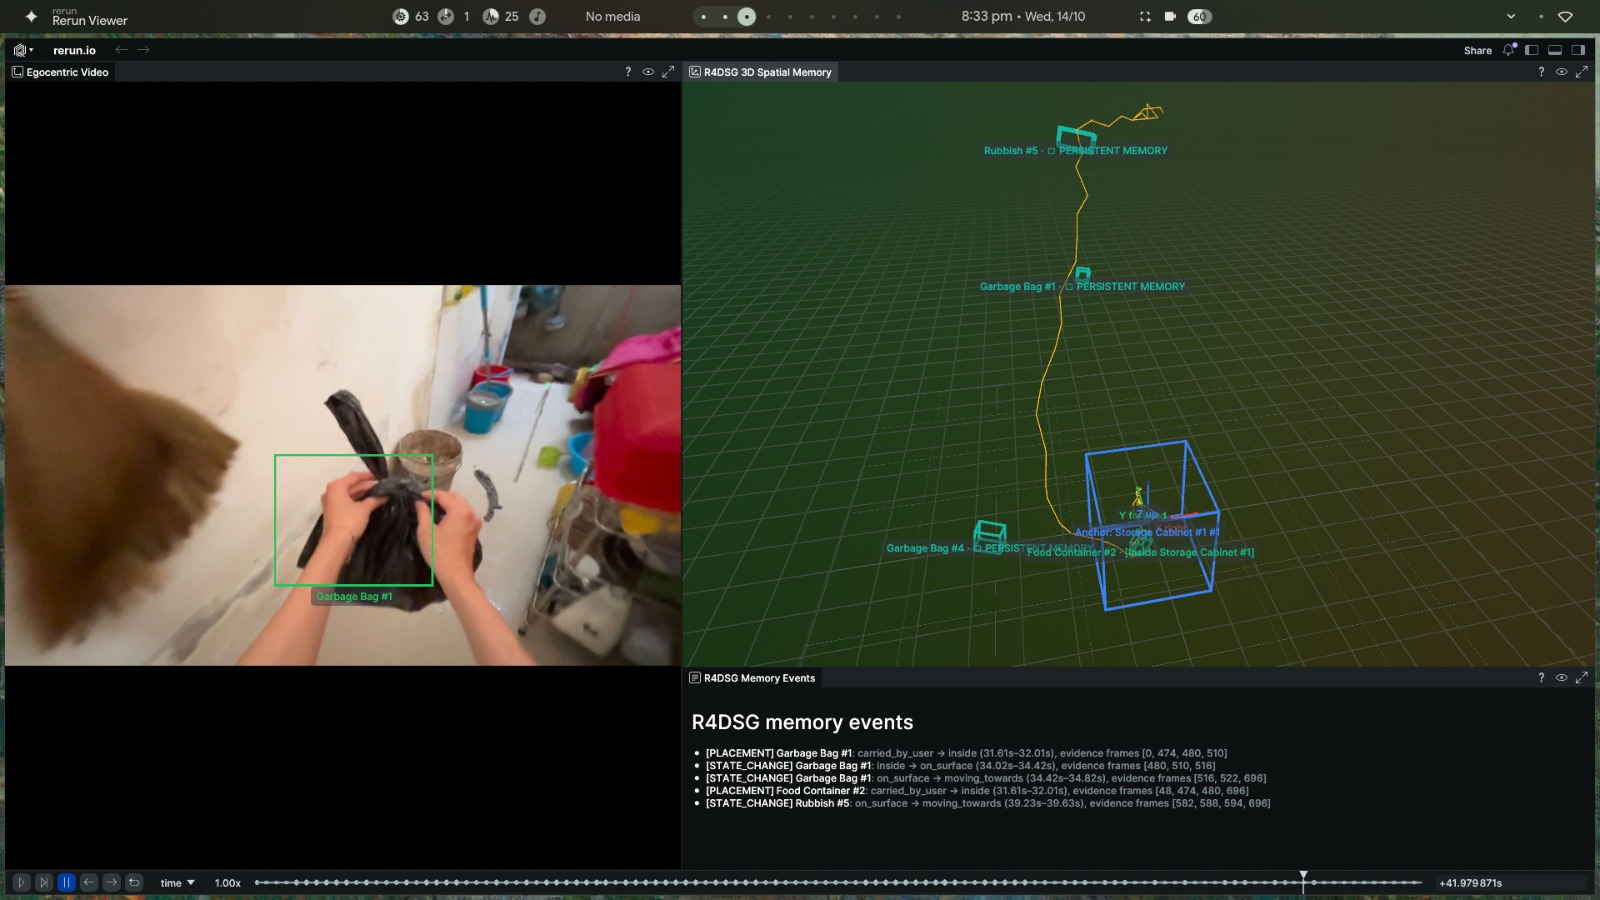
\includegraphics[width=\textwidth,height=0.55\textheight,keepaspectratio]{ThesisFigs/chapter6-screenshot-evidence.jpeg}\caption{Iteration~1 prototype screenshot (mid report).}\label{fig:screenshot-evidence}\end{figure}

\section{Iteration Outcome}
\label{sec:iter1-outcome}
The Iteration~1 artifact, API and client slice was implemented and tested in CI.
Its exit criteria were only partly evidenced: AC-06 (restart equivalence) and the
item query passed on fixtures, but no live capture reached memory, YOLOE missed
most small personal objects (it was replaced by SAM~3 in Iteration~2,
Section~\ref{sec:experiments}), and the per-frame timeline made the graph grow
with video length. These three findings set the Iteration~2 scope.

\chapter{Iteration 2: Design and Implementation}
\label{chap:iter2}
\textbf{Baseline.} This chapter covers work from 13~October to the end of FYP-1
on \texttt{develop} (commit \texttt{ce49dcc}, \tbd{update to the submission tag}).

\section{Iteration Objectives}
Iteration 2 had three objectives, taken from the Iteration~1 outcome and the
proposal feedback: (1) join live capture to memory, (2) make the memory bounded
and persistent across sessions (FR3.5, FR4), and (3) give the patient and
caregiver a usable product (proposal action 4). A fourth, unplanned objective
was to replace the detector after the benchmark of Section~\ref{sec:experiments}.

\section{Selected Use Cases / Features}
UC-01 (live), UC-03, UC-04, UC-06, UC-12 (compaction) and UC-13 (rooms) were
selected, plus UC-02 by speech, and the new UC-14 and UC-15.
Table~\ref{tab:i2-features} lists the features delivered.

\begin{table}[H]\centering\footnotesize
\caption{Iteration~2 features and their status.}\label{tab:i2-features}
\begin{tabularx}{\textwidth}{@{}Y L{3.6cm} L{2.0cm} l@{}}\toprule
\rowcolor{hdrfill}\textbf{Feature} & \textbf{Main files} & \textbf{FRs} & \textbf{Status}\\\midrule
Live capture contracts, keyframes, gaps, buffer, crash resume & \path{ingestion/live_pipeline.py}, \texttt{keyframe.py}, \texttt{buffer.py} & FR1, FR2 & Implemented\\
Promotion into segments and Modal runner & \texttt{live\_handoff.py}, \texttt{segment\_runner.py} & FR2.2 & Implemented\\
Gravity frame (RANSAC floor fit) & \path{geometry/gravity.py} & FR3.8 & Implemented\\
Nine relations in the gravity frame & \path{memory/relations.py} & FR3.8 & Implemented\\
State runs and events (schema 2) & \path{memory/runs.py}, \texttt{scene\_graph.py} & FR3.2, FR3.3 & Implemented\\
SQLite home store and cross-session matching & \texttt{store.py}, \texttt{matching.py}, \texttt{ingest.py} & FR3.5, FR3.9 & Implemented\\
Rooms, activities, room registry & \texttt{rooms.py}, \texttt{activities.py}, \texttt{home\_registry.py} & FR3.4, FR3.6 & Partial\\
Compaction with verification and roll-up & \texttt{compaction.py}, \texttt{summaries.py} & FR4 & Implemented\\
Evidence crops & \texttt{evidence.py} & FR7.2 & Implemented\\
SAM~3 detector, DINOv3 re-ID & \path{perception/detector.py} & FR3.1 & Implemented\\
Ranked candidates (tiered protocol) & \texttt{reasoning.py} & FR5.8 & Implemented\\
NLQ engine, dictionary (525 items), \path{/ask} & \path{nlq/engine.py}, \texttt{dictionary.py} & FR5.1, FR5.5 & Partial\\
Modal-served API & \path{remote/serve.py} & -- & Implemented\\
Patient App and Caregiver App & \texttt{apps/Patient App}, \texttt{apps/Caregiver App} & FR6, FR7, FR8.6, FR8.7 & Implemented (no auth)\\
Evaluation suite and EgoLife study & \path{evaluation/} & NFR-P & Implemented\\
\bottomrule\end{tabularx}\end{table}

\section{Design}
Figures~\ref{fig:i2-graph}--\ref{fig:i2-query} are the Iteration~2 class
diagrams, drawn from the code. Only fields and methods that matter to the design
are shown.

\aegisfig{ch7-class-memory-graph}{Memory graph classes (schema 2).}{fig:i2-graph}
\aegisfig{ch7-class-memory-runs}{Observations, state runs and events.}{fig:i2-runs}
\aegisfig{ch7-class-memory-store}{\texttt{HomeStore} and its records.}{fig:i2-store}
\aegisfig{ch7-class-memory-ingest}{Session ingest, matching and compaction.}{fig:i2-ingest}
\aegisfig{ch7-class-api-apps}{API models and the two Flutter apps.}{fig:i2-apps}
\aegisfig{ch7-class-query}{Query: ranking, NLQ engine and dictionary.}{fig:i2-query}

\clearpage
\section{Implementation}
This section describes the four algorithms added in Iteration~2.

\subsection{Relation classification}
\label{sec:relations-algo}
Each object box is compared with every anchor box in the gravity frame
(Figure~\ref{fig:flow-relations}). If gravity confidence is below 0.5 the
relation is \texttt{near} and marked uncertain. Otherwise, with a vertical
tolerance of 0.15 and a horizontal overlap threshold of 0.5, the classifier
decides in order: \texttt{carried} (a hand cue), \texttt{inside} (container
anchor, box within it), \texttt{on\_surface}, \texttt{under} (anchor open
underneath), \texttt{above}, \texttt{on\_floor} (within 6\% of the scene height
of the floor), \texttt{next\_to}, \texttt{near}, and finally \texttt{in\_room}.
Event types are \texttt{placed}, \texttt{picked\_up}, \texttt{moved},
\texttt{relation\_changed}, \texttt{room\_changed} and
\texttt{moved\_while\_unobserved}.

\aegisfigtall{ch7-flow-relations}{Relation classification flowchart.}{fig:flow-relations}

\subsection{State runs}
Observations of one instance are sorted by time. A run starts only when two
consecutive observations agree on anchor and relation (or one final observation
with confidence $\geq$ 0.5); instances with fewer than two observations are
dropped. Each change between runs gives one event. An object seen in the same
place for an hour is therefore one run, not 7{,}200 timeline rows.

\subsection{Cross-session matching}
\label{sec:matching-algo}
A new session is matched to the home in three levels
(Figure~\ref{fig:flow-matching}). \textbf{Rooms} match by landmark-signature
similarity (at least 0.5, a margin of 0.05 over the runner-up, at least one shared
landmark). \textbf{Anchors} are aligned by a rigid fit whose RMS residual must
stay below 25\% of the scene spread. \textbf{Objects} match by DINOv3 appearance
distance below 0.35 with a 0.1 margin; an object found at a different anchor
than its last-known state records \texttt{moved\_while\_unobserved}.

\aegisfig{ch7-flow-matching}{Cross-session matching flowchart.}{fig:flow-matching}

\subsection{Keyframe selection}
The live sampler keeps a frame (Figure~\ref{fig:flow-keyframe}) only if its mean
brightness is between 20 and 245, its Laplacian variance is at least 15 and its
change from the last kept frame (on a 64$\times$36 thumbnail) is at least 0.008;
a frame is forced after 2\,s without a keyframe so a still scene is still
recorded.

\aegisfig{ch7-flow-keyframe}{Keyframe selection flowchart.}{fig:flow-keyframe}

\subsection{Compaction}
Each local day (Asia/Karachi) older than three days is summarised by templates,
verified and only then deleted; important events stay seven days. Day summaries
older than 30 days roll up into weeks, and weeks older than 365 days into months.
The last-known run and evidence crop of every object are kept.

\section{Technical Implementation Details}
Table~\ref{tab:params} lists the defaults in \path{core/config.py}. All are
overridable from \path{configs/*.yaml}.

\begin{table}[H]\centering\footnotesize
\caption{Main Iteration~2 parameters.}\label{tab:params}
\begin{tabularx}{\textwidth}{@{}L{4.6cm} l Y@{}}\toprule
\rowcolor{hdrfill}\textbf{Parameter} & \textbf{Default} & \textbf{Effect}\\\midrule
\texttt{live.sample\_fps} & 2.0 & Frames sampled from MJPEG\\
\texttt{live.max\_duration\_seconds} & 600 & Session limit\\
\texttt{live.reconnect\_timeout\_seconds} & 30 & End after this long without frames\\
\texttt{live.buffer\_capacity} & 30 & Frames held during a stall\\
\texttt{live.segment\_frames} & 120 & Frames per promoted segment\\
\texttt{max\_gap\_seconds} & 30 & Gap that splits a segment\\
\texttt{memory.anchor\_cluster\_radius} & 0.40 & Anchor clustering (VGGT units)\\
\texttt{memory.association\_radius} & 0.45 & Same-instance radius\\
\texttt{memory.appearance\_threshold} & 0.35 & DINOv3 distance for re-ID\\
\texttt{memory.min\_run\_observations} & 2 & Debounce for a new run\\
\texttt{compaction.hot\_days} / \texttt{important\_hot\_days} & 3 / 7 & Detail retention\\
\texttt{compaction.weekly\_rollup\_after\_days} / \texttt{monthly\_\ldots} & 30 / 365 & Roll-up\\
\texttt{evidence.max\_side}, \texttt{quality} & 320, 85 & Crop size and JPEG quality\\
\bottomrule\end{tabularx}\end{table}

Set-up and the main commands (from \texttt{README.md}):
\begin{verbatim}
uv sync                                  # install
uv run pytest                            # 451 tests, coverage floor 75%
uv run aegis-ingest --url http://<phone>:8080/video
uv run python run_pipeline.py --live-session <id>
modal deploy src/aegis/remote/serve.py   # aegis-memory-api
uv run aegis-ask "where are my keys?"
\end{verbatim}

\section{Tools, Frameworks and Technologies}
In addition to the Iteration~1 stack: SAM~3 (default detector), DINOv3
(re-identification), SQLite, the Flutter \texttt{speech\_to\_text} plugin
(on-device speech), and \texttt{matplotlib} and PlantUML for the report figures.
Tools used for writing and coding are disclosed in Section~\ref{sec:tools}.

\section{Demonstration Evidence}
\tbd{Screenshots to be added by the team: Patient App home and answer sheet,
Caregiver App Interior and Track tabs, Rerun view of walk01-2, and a terminal
run of \texttt{run\_pipeline.py}.}

\section{Iteration Outcome}
\label{sec:iter2-outcome}
Objectives (1)--(3) were met as implemented slices. A live capture now reaches
memory on Modal (end-to-end run of 20~November, Section~\ref{sec:e2e}); memory is
bounded (5.7--7.2$\times$ smaller, 100\% retention of last-known states,
Section~\ref{sec:compaction-audit}) and persists across sessions (12/12 instances
still found 1--4 days later on EgoLife, Section~\ref{sec:egolife}); and both apps
are built and tested. Not met: temporal answers (FR5.2, deviation D2),
calibrated abstention, authentication (FR8.1), encryption, the one-hour soak,
latency p95 and any user study. Room linking proved unstable across scale
(TC12). These items form Iteration~3 and~4 (Chapter~\ref{chap:fyp2}).

\chapter{Testing and Validation}
\label{chap:testing}

\section{Testing Strategy}
Testing has four levels (Figure~\ref{fig:test-levels}). Unit and integration
tests run in CI on every push and gate merges; evaluation scripts run on real or
synthetic data and produce reports; system runs exercise the deployed pipeline;
acceptance is judged against the checks of Table~\ref{tab:ac}. A result is
called \emph{measured} only when a script produced it from data; otherwise it is
\emph{unmeasured}.

\aegisfig{ch8-test-levels}
  {Test levels with the number of tests or runs at each level at the end of FYP-1.}
  {fig:test-levels}

\section{Test Levels and Results}
\textbf{Unit and integration.} \texttt{uv run pytest} collects 451 tests in 53
files; all pass. Line coverage is 79\% of 10{,}759 statements, above the 75\% CI
floor. Ruff lint and format checks pass. The Flutter apps have 14 (Patient) and
11 (Caregiver) widget tests. Appendix~\ref{app:tests} lists the tests by file.

\textbf{Detection.} The detector benchmark is reported in
Table~\ref{tab:detector-ab}: SAM~3 reached F1~0.721 against YOLOE's 0.097 on
the same labelled frames, and found 34 of 42 shoes and all 19 hands. SAM~3 still
produces 3.3 false positives per image, so the memory relies on debouncing (two
agreeing observations) to suppress them.

\section{Compaction and Storage Audit}
\label{sec:compaction-audit}
The memory audit (\path{evaluation/memory_audit.py}) compares the schema-1
per-frame graph with the schema-2 state-run graph for the same session and
checks that every last-known state survives. Figure~\ref{fig:compaction-ratio}
shows the result: \texttt{demo04} shrank 7.2$\times$ (178.3 to 24.8\,KiB) and
\texttt{demo03} 5.7$\times$ (528.5 to 92.0\,KiB), with 100\% retention of
last-known states. Projected to continuous use (Figure~\ref{fig:storage-projection}),
\texttt{demo04} grows at 2.11\,MiB/h instead of 13.51\,MiB/h, i.e.\ 50.7\,MiB
instead of 324.2\,MiB per 24 hours, before compaction of old days. The projection
is linear from short clips and is not a long-run measurement (P2.8).

\aegisfig{ch8-compaction-ratio}{Graph size before and after state runs, and retention.}{fig:compaction-ratio}
\aegisfig{ch8-storage-projection}{Projected storage growth for 24 hours.}{fig:storage-projection}

\section{End-to-End System Run}
\label{sec:e2e}
On 20~November \path{scripts/run_e2e.py} ran the full pipeline on the
\texttt{walk01-2} capture (79 frames) with CPU containers. VGGT took 831\,s,
detection and lifting 27\,s, and deployment of the API 8\,s
(Figure~\ref{fig:e2e-timing}); the API then answered queries from the volume.
The run proves the stages connect; it is not a latency measurement, because a GPU
run would be much faster and only one run was made.

\aegisfig{ch8-e2e-timing}{Stage timings of the end-to-end run (CPU, 79 frames).}{fig:e2e-timing}

At the measured L4 rate a 5-minute segment costs 0.086 GPU-hours, about
\$0.069.

\section{EgoLife Multi-Day Study}
\label{sec:egolife}
Because Ego4D could not be used (NO\_GO: 0 of 100 sampled clips were usable, and
the prerequisites would take about 10.8 weeks), memory persistence was tested on
EgoLife, a seven-day egocentric recording. 74 segments were processed for
\$8.71. Two results matter. First, 12 of 12 tracked instances were still in the
store 1--4 days after they were last seen, so the store does not forget across
days. Second, using the full history never answered better than an ablation that
used only the last 24 hours, so on this data long history did not help
answering. A defect found here is listed in Table~\ref{tab:defects} (D-4).
\tbd{Per-day table (segments, objects, rooms, queries correct) and the F8.6
figure to be added from the team's EgoLife run notes.}

\section{Acceptance Testing}
Of the 35 acceptance checks (Table~\ref{tab:ac}), 7 pass, 10 pass partly, 1
fails (AC-20, no encryption at rest) and 17 have not been run. Every check that
has not been run is listed with its FYP-2 task (P-numbers in
Chapter~\ref{chap:fyp2}).

\section{Edge and Failure Cases}
Tested edge cases include: unknown items and unknown words (specific abstention
codes); several same-class objects (ambiguous, up to three photos); an object
never observed; a server timeout in the apps; a stream disconnect and reconnect;
a storage stall with a full buffer; a crash and resume from
\texttt{session\_state.json}; a corrupt \texttt{home\_map.json}; a duplicate room
label; an unchanged graph re-ingested (skipped by SHA-256); a failed summary
verification (detail kept); and a gravity fit with low confidence (relation
marked uncertain).

\section{Defects and Corrective Actions}
\begin{table}[H]\centering\footnotesize
\caption{Defects found in Iteration~2 and their fixes.}\label{tab:defects}
\begin{tabularx}{\textwidth}{@{}l Y Y l@{}}\toprule
\rowcolor{hdrfill}\textbf{\#} & \textbf{Defect} & \textbf{Correction} & \textbf{Commit}\\\midrule
D-1 & YOLOE missed most personal objects (F1 0.097) & SAM~3 made the default & \tbd{[ ]}\\
D-2 & Per-frame timeline grew with video length & State runs, schema 2 & \texttt{0bfc257}\\
D-3 & Display transform (SCALE, \texttt{to\_zup}) hid real geometry & Raw coordinates + gravity frame & \tbd{[ ]}\\
D-4 & EgoLife DAY7: rooms 44 $\rightarrow$ 40 and anchors 859 $\rightarrow$ 818 after re-ingest (duplicate identities) & Matching fix & \texttt{61dda40}\\
D-5 & Apps showed a mock answer when offline & Mock removed; ``Can't reach Aegis memory'' & \texttt{180b897}\\
D-6 & Room linking unstable across scene scale (TC12) & Open: scale-relative linking (Iteration~3) & --\\
\bottomrule\end{tabularx}\end{table}

\section{Measured and Unmeasured Results}
\textbf{Measured:} test count and coverage; detector F1; compaction ratio and
retention; storage projection (from short clips); end-to-end stage times (one
CPU run); EgoLife persistence and the 24-hour ablation; GPU cost per segment.
\textbf{Unmeasured:} spatial and temporal retrieval accuracy (NFR-P4, AC-09/10;
\texttt{demo05} is NOT\_READY), the four room metrics, query latency p95
(NFR-P1), the one-hour soak (NFR-R1), speech accuracy, and usability. These are
not reported as results anywhere in this report.

\chapter{Project Management and Development Evidence}
\label{chap:pm}

\section{Work Completed and Remaining}
Completed work is listed in Table~\ref{tab:i2-features} (Iteration~2) and
Section~\ref{sec:iter1-outcome} (Iteration~1). Remaining work is the FYP-2 plan
of Chapter~\ref{chap:fyp2}.

\section{Contribution of Each Team Member}
Table~\ref{tab:contributions} uses Git author identities on all branches
(non-merge commits). Commit counts are a repository metric, not a measure of
effort or quality: one commit may be one line or a whole module, and on
23~November 122 of Ali Sher's commits each added a single app file.

\begin{table}[H]\centering\footnotesize
\caption{Contribution evidence from Git history.}\label{tab:contributions}
\begin{tabularx}{\textwidth}{@{}L{2.6cm} L{3.2cm} l Y@{}}\toprule
\rowcolor{hdrfill}\textbf{Member} & \textbf{Git identity} & \textbf{Commits} & \textbf{Main areas evidenced}\\\midrule
Shahmeer Amir & \texttt{shah-paradox} & 47 & Live capture contracts, keyframes, gaps and buffer; the M1/M2 pass (gravity, relations, state runs, store, rooms, compaction, segment runner); Part~II plan; report and diagrams\\
Faizan ur Rehman Khan & \texttt{pez-Ox}, \texttt{Faizan Ur Rehman Khan} & 57 + 1 & Batch pipeline and R4DSG baseline; CI/CD and API; in-hand memory and Rerun; room hierarchy and registry; evaluation suite; demo harness; EgoLife study; tiered query protocol; SAM~3 benchmark\\
Ali Sher & \texttt{Ali Sher}, \texttt{Ali-Sher12} & 218 & Flutter redesign and search history; NLQ engine and \path{/ask}; Modal-served API; end-to-end runner; Patient and Caregiver Apps; enrolment; DINOv3 re-ID\\
\bottomrule\end{tabularx}\end{table}
\tbd{Each member to confirm their row and lead modules.}

\section{Milestones and Commit Evidence}
Figure~\ref{fig:commit-timeline} shows commits per week and member;
Figure~\ref{fig:branch-graph} shows the branches and the two tags. Work was
concentrated in two bursts: the mid-evaluation (weeks 40--42) and Iteration~2
(weeks 45--48).

\aegisfig{ch9-commit-timeline}{Commits per ISO week and author (non-merge).}{fig:commit-timeline}
\aegisfig{ch9-branch-graph}{Branches, merges and tags.}{fig:branch-graph}

\section{Repository and Version Control}
The repository uses a \texttt{src} layout (\path{src/aegis/}), YAML
configuration in \path{configs/}, tests in \path{tests/}, the apps in
\path{apps/}, and conventional commit messages. Work happens on feature
branches merged into \texttt{develop}; \texttt{main} receives tagged releases
(\texttt{v0.1.0-mid1}, \texttt{v0.2.0-mid2}). CI runs Ruff, pytest with the
coverage floor and Flutter checks. Appendix~\ref{app:repository} gives the
layout.

\section{Tools and Tool-Assisted Development}
\label{sec:tools}
VGGT-$\Omega$, SAM~2, SAM~3, DINOv3, YOLOE, FastAPI, Flutter, Modal, OpenCV and
Rerun are external components. AI assistants were used for coding help, for
drafting parts of this report in LaTeX and for diagram markup (PlantUML and
matplotlib scripts). The team reviewed all generated material and is responsible
for the architecture, algorithms, requirements, tests and claims.
\tbd{Per-member disclosure of which assistant was used for what, to be completed
by each member.}

\section{External Components and Dependencies}
\begin{table}[H]\centering\footnotesize
\caption{External dependencies.}\label{tab:external-dependencies}
\begin{tabularx}{\textwidth}{@{}L{4.6cm} Y l@{}}\toprule
\rowcolor{hdrfill}\textbf{Dependency} & \textbf{Use} & \textbf{Status}\\\midrule
Python 3.12, uv, NumPy, OpenCV, PyYAML & Runtime and video processing & Used\\
FastAPI, Uvicorn, httpx & API and tests & Used\\
SQLite (standard library) & Home store & Used\\
Modal, CUDA images, L4 GPU & Remote workers and API hosting & Used\\
VGGT-$\Omega$ & Poses and 3D points & Used\\
SAM~3, YOLOE, SAM~2 & Detection and masks & Used\\
DINOv3 & Re-identification & Used\\
Flutter/Dart, \texttt{speech\_to\_text} & Apps and on-device speech & Used\\
Rerun & Offline 3D viewer & Optional\\
Hugging Face Hub & Model weights (gated VGGT-$\Omega$, mirror fallback) & Used\\
Identity provider, encryption library & Authentication and encryption at rest & Planned\\
\bottomrule\end{tabularx}\end{table}

\section{Risks and Mitigation}
Likelihood (L) and impact (I) are scored 1--3; the score is L$\times$I.
\begin{table}[H]\centering\footnotesize
\caption{Scored risk register.}\label{tab:risk-register}
\begin{tabularx}{\textwidth}{@{}l Y l l l Y@{}}\toprule
\rowcolor{hdrfill}\textbf{ID} & \textbf{Risk} & \textbf{L} & \textbf{I} & \textbf{Score} & \textbf{Mitigation / status}\\\midrule
TC1 & Identity errors under clutter and occlusion & \tbd{2} & \tbd{3} & \tbd{6} & DINOv3 re-ID, debouncing; matching fix 61dda40\\
TC2 & Compaction loses useful detail & \tbd{1} & \tbd{3} & \tbd{3} & Verification before delete; last-known protected\\
TC3 & Motion blur and lighting & \tbd{2} & \tbd{2} & \tbd{4} & Keyframe gate\\
TC4 & GPU cost and latency & \tbd{2} & \tbd{2} & \tbd{4} & L4 \$0.069 per 5-min segment; CPU fallback\\
TC5 & Hallucinated answers & \tbd{1} & \tbd{3} & \tbd{3} & Closed-vocabulary rule engine; abstention codes\\
TC6 & High interaction load for older users & \tbd{2} & \tbd{2} & \tbd{4} & Object tiles, large targets; usability study planned\\
TC7 & Privacy and consent & \tbd{3} & \tbd{3} & \tbd{9} & Open: auth, encryption (Iteration~4)\\
TC8 & Limited validation & \tbd{3} & \tbd{2} & \tbd{6} & Measured/unmeasured separation; \texttt{demo05}\\
TC9 & Evaluation dataset & \tbd{2} & \tbd{2} & \tbd{4} & Ego4D NO\_GO; EgoLife used\\
TC10 & RGB-only spatial uncertainty & \tbd{2} & \tbd{2} & \tbd{4} & Gravity frame; no metric claims\\
TC11 & Room errors and cross-session identity & \tbd{2} & \tbd{2} & \tbd{4} & Registry, matching; metrics planned\\
TC12 & Room linking unstable across scale & \tbd{3} & \tbd{2} & \tbd{6} & Scale-relative linking (Iteration~3)\\
\bottomrule\end{tabularx}\end{table}

\section{Security and Privacy Considerations}
\label{sec:security}
The current prototype is not safe for real patient data. The API has no
authentication or authorisation; CORS allows any origin, method and header; the
writes \path{/rooms/rename}, \path{/enroll}, \path{/dataset/select} and
\path{/capture/pause} are open; and \texttt{GET /video/\{dataset\_id\}} serves
raw video to anyone with the URL. The home store, \texttt{home\_map.json} and
evidence crops are stored unencrypted. HTTPS is provided only by the Modal
endpoint. Speech is transcribed on the phone, so no audio leaves it. All testing
used team-recorded or public data. Iteration~4 addresses these gaps (P1.7, P1.8).

\section{Current Limitations}
Spatial and temporal accuracy, latency and usability are unmeasured; temporal
answers are not built; confidence is not calibrated; room linking is unstable
across scale; storage growth is projected from short clips; and no clinical
claim is made.

\chapter{Remaining FYP Plan}
\label{chap:fyp2}

\section{Remaining Scope}
FYP-2 completes the parts of FYP-1 that were not met (Section~\ref{sec:iter2-outcome})
and measures what is still unmeasured (Section~\ref{sec:egolife} onward). It adds
no new modules.

\section{Remaining Iterations}
\textbf{Iteration 3} finishes the query engine and evaluation data: temporal
answers (P1.1), calibrated confidence (P1.2), freshness (P1.3), evidence
references (P1.4), multi-instance clarification and a query log (P1.5), a speech
confirmation step (P1.6), scale-relative room linking (the TC12 fix), annotation
and scoring of \texttt{demo05} (P2.5) and the room metrics (P2.3).
\textbf{Iteration 4} covers security and validation: authentication, grants,
consent, audit and a restricted CORS policy (P1.7), encryption and full deletion
(P1.8), an optional LLM planner (P1.9), the one-hour soak and disconnect tests
(P2.1), placement and activity ground truth (P2.2), a controlled room (P2.4),
latency p95 and compaction before/after (P2.8), a 7- and 30-day persistence pilot
(P2.7), a usability study after ethics approval, and the thesis.

\aegisfig{ch10-fyp2-gantt}{FYP-2 plan by iteration. Dates and owners are team input.}{fig:fyp2-gantt}

\begin{table}[H]\centering\footnotesize
\caption{FYP-2 work packages.}\label{tab:fyp2}
\begin{tabularx}{\textwidth}{@{}l Y l l l@{}}\toprule
\rowcolor{hdrfill}\textbf{Iter.} & \textbf{Work} & \textbf{Closes} & \textbf{Owner} & \textbf{Dates}\\\midrule
3 & Temporal answers, confidence, freshness, evidence refs & FR5.2--5.5, AC-10, AC-11 & \tbd{[ ]} & \tbd{[ ]}\\
3 & Clarification, query log, speech confirmation & FR5.8, FR6.3 & \tbd{[ ]} & \tbd{[ ]}\\
3 & Scale-relative room linking; room metrics & FR3.6, AC-22 & \tbd{[ ]} & \tbd{[ ]}\\
3 & \texttt{demo05} annotation and scoring & NFR-P4, AC-09 & \tbd{[ ]} & \tbd{[ ]}\\
4 & Auth, grants, consent, audit, CORS & FR8.1--8.5, AC-16--18, AC-26 & \tbd{[ ]} & \tbd{[ ]}\\
4 & Encryption and deletion & NFR-S1, NFR-S5, AC-20 & \tbd{[ ]} & \tbd{[ ]}\\
4 & Soak, latency, compaction measurements & NFR-R1, NFR-P1, AC-19, AC-33 & \tbd{[ ]} & \tbd{[ ]}\\
4 & Persistence pilot; usability study & NFR-U1, AC-15 & \tbd{[ ]} & \tbd{[ ]}\\
\bottomrule\end{tabularx}\end{table}

\section{Testing and Validation Plan}
Each FYP-2 package ends with a test in CI or an evaluation script whose output is
reported; nothing is reported as a result without one. The targets are those of
Section~\ref{sec:success}: spatial retrieval at least 70\%, temporal at least
60\%, p95 latency within NFR-P1, and a one-hour soak without crash.

\section{Deployment Plan}
The deployment of Figure~\ref{fig:deployment} stays. Iteration~4 adds
authentication in front of the API, restricts CORS to the two apps, closes the
raw-video route and encrypts the store at rest.

\section{Expected Final Deliverables}
A reproducible repository with tagged releases, the two apps, the deployed API,
evaluation reports with the measured results above, the final presentation and
the thesis. A clinical efficacy claim is not a deliverable.

\chapter{Conclusion}
\label{chap:conclusion}
Aegis set out to answer ``where did I leave it?'' for a person with memory
impairment from first-person video. At the end of FYP-1 the whole path exists: a
phone streams video, a laptop keeps sharp, new frames and uploads segments,
Modal reconstructs them in 3D and detects objects, the memory records where each
object is relative to furniture and rooms in a bounded, persistent per-home
store, and two apps let the patient and caregiver ask by tapping, typing or
speaking, with a photo as evidence. 451 tests pass with 79\% coverage.

Three results stand out. SAM~3 made small personal objects detectable (F1 0.721
against 0.097). State runs made memory bounded (5.7--7.2$\times$ smaller with no
loss of last-known states). And the store kept every tracked object across days
on EgoLife.

The report is equally clear about what is not done. Temporal answers,
calibrated confidence, authentication and encryption are not built; accuracy,
latency and usability are not measured; and the prototype is not safe for
patient data. FYP-2 (Chapter~\ref{chap:fyp2}) closes these gaps and measures
the results before any claim is made.

\appendix
\chapter{Proposal Action Register}
\label{app:actions}
\textbf{Update at the end of FYP-1.} The status of each action is now given, with its evidence, in the action register of Chapter~\ref{chap:plan}. The text below is the response as written at the mid report and is kept for the record.


This appendix records the panel's required proposal changes and the response
supported by the report. Status distinguishes written clarification from
implemented or evaluated work.

\begin{enumerate}
\item \textbf{Narrow the scope and define persistence.} Chapter~1 specifies a
three-day structured spatial-memory objective, with older spatial observations
to be converted into text summaries. The retention/compaction policy has not
been implemented or evaluated. \emph{Status: partially addressed; implementation
and evaluation remain planned.}

\item \textbf{Define the complex computing problem and acceptance criteria.}
Chapter~2 explains the fidelity--storage trade-off; Chapters~1 and~4 define
proposed success criteria and acceptance checks. Room metrics are targets, not
measured results. \emph{Status: addressed in the report; evaluation pending.}

\item \textbf{State compute, storage and device assumptions.} Chapter~1 records
the development laptops, mobile RGB capture device and Modal L4 inference
assumption. Resource assumptions are documented, but a complete resource
benchmark is outstanding. \emph{Status: partially addressed.}

\item \textbf{Improve the application design and UI/UX.} The report includes
the redesigned Flutter patient/caregiver views and wireframes. No usability
study or validation with intended users is reported, and no room-calibration
screen is implemented. \emph{Status: partially addressed.}
\end{enumerate}

The detailed proposal response appears in Chapter~3, Section~3.2. Remaining
implementation and validation work is summarized in Chapter~10.
\chapter{Supplementary Use-Case Specifications}
\label{app:usecases}

The principal use cases are specified in Chapter~4. This appendix provides the
remaining use-case flows referenced by its use-case inventory. Requirements are
specified behaviour; notes on current implementation distinguish working
slices from planned behaviour.

\section{Query and Recall Use Cases}
\subsection{UC-02: Submit a Query by Speech or Text}
\uctable{UC-02 detail.}
{Primary user}
{The application and memory service are available. Typed queries are supported; speech is transcribed on the device when available (both apps, since 23 November).}
{The user enters or speaks a question about an object or past activity.}
{1.~The interface accepts a typed query. 2.~The query service extracts the target and any room constraint. 3.~The service retrieves matching memory and evidence. 4.~The interface displays the grounded response.}
{A1: Speech transcription is unavailable or uncertain $\rightarrow$ the user may enter the query as text. A2: No supporting memory exists $\rightarrow$ the service returns a not-found response rather than inventing a location.}
{The query and its response are displayed.}
{FR5, FR6, FR7}

\subsection{UC-04: Review the History of an Object}
\uctable{UC-04 detail.}
{Primary user; caregiver access is a future authorized role}
{The scene graph contains one or more observations of the requested object.}
{The user opens the timeline or asks to review an object's earlier locations.}
{1.~The client requests the timeline. 2.~The service returns timestamped observations/events. 3.~The user reviews the ordered history and its room/anchor context when available.}
{A1: No history is found $\rightarrow$ the interface reports that no observation is available. A2: An object is ambiguous $\rightarrow$ the user selects the desired instance.}
{The chronological history is shown with available location and time evidence.}
{FR3, FR4, FR5, FR7}

\subsection{UC-06: View Evidence for an Answer}
\uctable{UC-06 detail.}
{Primary user}
{A query has produced an answer or an explicit not-found result.}
{The user opens the answer details.}
{1.~The interface displays the short answer. 2.~It shows the supporting description/image reference, timestamp, anchor and room fields when available. 3.~The user can distinguish a stored observation from a missing-evidence response.}
{A1: Evidence is unavailable $\rightarrow$ the response identifies the missing evidence and does not present an unsupported location as fact.}
{The answer is presented with its available provenance.}
{FR5.4, FR7.2}

\section{Caregiver and Memory-Maintenance Use Cases}
\subsection{UC-08: Caregiver Queries Episodic History}
\uctable{UC-08 detail.}
{Caregiver; authentication and authorization are specified requirements but are not implemented}
{A memory service and relevant history exist. The current API does not establish a verified caregiver identity or patient boundary.}
{A caregiver requests an object-state answer or activity summary within the primary user's granted scope; unrestricted raw-history browsing is outside the caregiver role.}
{1.~The caregiver requests an object-state answer or activity summary. 2.~The service checks the granted scope when authorization is implemented. 3.~It retrieves only the in-scope information and returns a concise response with evidence.}
{A1: No matching observation exists $\rightarrow$ return an explicit not-found response. A2: The request is outside an authorized scope $\rightarrow$ deny it when access control is implemented; current authorization enforcement is absent.}
{A grounded response is returned by the current query service; secure caregiver access remains future work.}
{FR5, FR8}

\subsection{UC-10: Caregiver Reviews an Activity Summary}
\uctable{UC-10 detail.}
{Caregiver}
{A summary for the selected period exists and the caregiver has authenticated access. Summary generation and caregiver authorization are not implemented in the current prototype.}
{The caregiver requests a daily activity summary.}
{1.~The client requests the selected date. 2.~The system gathers timestamped events and any available room/object context. 3.~It presents a concise summary with evidence references.}
{A1: No events are available $\rightarrow$ report that the interval has no recorded activity. A2: The interval contains only compacted data $\rightarrow$ label summary-derived content as summarized.}
{The requested summary is displayed with its evidence level; this use case remains planned.}
{FR3, FR4, FR8}

\subsection{UC-11: Pause Capture or Delete History}
\uctable{UC-11 detail.}
{Primary user}
{A capture session or stored memory exists.}
{The user pauses capture or requests deletion of stored history.}
{1.~The user selects pause or delete. 2.~The system stops accepting new capture while paused, or confirms the deletion request. 3.~For deletion, the system removes the selected stored history and reports completion.}
{A1: Capture is already paused $\rightarrow$ keep it paused. A2: Deletion cannot be verified $\rightarrow$ report the failure rather than claim success.}
{The user receives the capture/deletion state. Full deletion and production safeguards remain requirements, not demonstrated safeguards.}
{FR1.3, NFR-S5}

\subsection{UC-12: Maintain Memory by Compaction}
\uctable{UC-12 detail.}
{System}
{A home store exists with days older than \texttt{hot\_days} (3).}
{A home ingest completes (compaction runs after every ingest).}
{1.~For each local day older than three days (seven for important events), the system builds template summaries. 2.~It verifies each summary against its source rows. 3.~Only then does it delete the detail rows, keeping every object's last-known run and evidence. 4.~Day summaries older than 30 days roll up into weeks, and weeks older than 365 days into months. 5.~Timeline answers from summaries carry \texttt{tier}.}
{A1: Verification fails $\rightarrow$ the day keeps all detail and \texttt{compaction\_log} records \texttt{failed}.}
{Older history is queryable as summaries; last-known states are unchanged. Implemented (\texttt{memory/compaction.py}, 14 tests); accuracy after compaction is unmeasured.}
{FR4.1--FR4.5}

\section{Use-Case Coverage}
UC-01, UC-03, UC-05, UC-07, UC-09, UC-13 and UC-14 are detailed in Chapter~4. This appendix details UC-02,
UC-04, UC-06, UC-08, UC-10, UC-11 and UC-12. The use-case inventory and
requirements traceability matrix in Chapter~4 provide the complete ID-to-FR
mapping.
\chapter{Detailed Test Cases and Results}
\label{app:tests}
Table~\ref{tab:app-tests} lists every Python test file with its number of test functions (parametrised tests expand to the 451 collected tests). All pass on \texttt{develop}; line coverage is 79\%. The Flutter apps add 14 (Patient App) and 11 (Caregiver App) widget tests. These are unit and integration checks; system and acceptance results are in Chapter~\ref{chap:testing}.

\begin{ltab}\footnotesize
\begin{longtable}{@{}L{4.0cm}L{6.4cm}r@{}}
\caption{Test files by area.}\label{tab:app-tests}\\
\toprule
\rowcolor{hdrfill}\textbf{Area} & \textbf{File} & \textbf{Tests}\\
\midrule
\endfirsthead
\toprule
\rowcolor{hdrfill}\textbf{Area} & \textbf{File} & \textbf{Tests}\\
\midrule
\endhead
\bottomrule
\endfoot
Capture and ingestion & \texttt{test\_capture\_control.py} & 2\\
 & \texttt{test\_config.py} & 10\\
 & \texttt{test\_live\_buffer.py} & 3\\
 & \texttt{test\_live\_cli.py} & 8\\
 & \texttt{test\_live\_contracts.py} & 12\\
 & \texttt{test\_live\_handoff.py} & 8\\
 & \texttt{test\_live\_ingestion.py} & 13\\
 & \texttt{test\_live\_keyframe.py} & 6\\
 & \texttt{test\_live\_segments.py} & 7\\
 & \texttt{test\_video\_ingestion.py} & 5\\
 & \texttt{test\_wallclock.py} & 4\\
\midrule
Geometry and perception & \texttt{test\_detector\_postprocess.py} & 6\\
 & \texttt{test\_geometry.py} & 5\\
 & \texttt{test\_gravity.py} & 11\\
 & \texttt{test\_lifting.py} & 15\\
 & \texttt{test\_planar.py} & 6\\
 & \texttt{test\_vggt\_checkpoint.py} & 3\\
\midrule
Memory & \texttt{test\_activities.py} & 7\\
 & \texttt{test\_anchors.py} & 4\\
 & \texttt{test\_association.py} & 6\\
 & \texttt{test\_compaction.py} & 14\\
 & \texttt{test\_evaluation\_controlled\_room.py} & 3\\
 & \texttt{test\_evidence.py} & 7\\
 & \texttt{test\_home\_registry.py} & 4\\
 & \texttt{test\_ingest.py} & 12\\
 & \texttt{test\_matching.py} & 15\\
 & \texttt{test\_relations.py} & 5\\
 & \texttt{test\_repository.py} & 4\\
 & \texttt{test\_restart\_equivalence.py} & 3\\
 & \texttt{test\_room\_identity.py} & 6\\
 & \texttt{test\_rooms.py} & 9\\
 & \texttt{test\_runs.py} & 5\\
 & \texttt{test\_scene\_graph.py} & 18\\
 & \texttt{test\_store.py} & 4\\
 & \texttt{test\_vocabulary.py} & 12\\
\midrule
Query and API & \texttt{test\_api.py} & 28\\
 & \texttt{test\_modal\_compute.py} & 1\\
 & \texttt{test\_nlq.py} & 9\\
 & \texttt{test\_ranking.py} & 12\\
 & \texttt{test\_reasoning.py} & 12\\
 & \texttt{test\_serve\_app.py} & 2\\
\midrule
Evaluation and demo & \texttt{test\_demo\_calibrate.py} & 4\\
 & \texttt{test\_demo\_harness.py} & 7\\
 & \texttt{test\_egolife.py} & 30\\
 & \texttt{test\_evaluation\_memory\_audit.py} & 4\\
 & \texttt{test\_evaluation\_metrics.py} & 13\\
 & \texttt{test\_evaluation\_option\_c.py} & 6\\
 & \texttt{test\_evaluation.py} & 6\\
 & \texttt{test\_evaluation\_query.py} & 8\\
 & \texttt{test\_evaluation\_run.py} & 1\\
 & \texttt{test\_mid1\_prototype.py} & 4\\
 & \texttt{test\_rerun\_visualization.py} & 3\\
 & \texttt{test\_run\_e2e.py} & 13\\

\end{longtable}
\end{ltab}

\chapter{Repository and Contribution Evidence}
\label{app:repository}

The repository and contribution evidence summarized here has also been presented in the report's Chapter~9, Project Management and Development Evidence. This appendix provides the supporting repository paths and reproduction details.

\section{Repository Layout}
The project is maintained in the \texttt{aegis} repository. The main source
modules and their roles are:

\begin{table}[H]\centering\small
\caption{Principal repository paths.}\label{tab:appendix-repository}
\begin{tabularx}{\textwidth}{@{}L{4.8cm}Y@{}}\toprule
\textbf{Path}&\textbf{Contents}\\\midrule
\path{src/aegis/core/}&Runtime configuration, typed models and canonical paths.\\
\path{src/aegis/geometry/}&VGGT-$\Omega$ reconstruction, coordinate/point utilities and 2D-to-3D lifting.\\
\path{src/aegis/perception/}&Open-vocabulary object and room-landmark detection/segmentation.\\
\path{src/aegis/memory/rooms.py}&Trajectory-based room regions, footprints, labels and room assignment.\\
\path{src/aegis/memory/home_registry.py}&Per-home room identity records persisted as \texttt{home\_map.json}.\\
\path{src/aegis/memory/scene_graph.py}&Rooms--Anchors--Objects bindings, observations and temporal events.\\
\path{src/aegis/memory/reasoning.py}&Object/room query parsing and grounded explanations.\\
\path{src/aegis/remote/api.py}&FastAPI query, graph, timeline, room-list and room-rename routes.\\
\path{src/aegis/remote/workers.py}&Pipeline workers and Rerun logging, including room depictions.\\
\bottomrule\end{tabularx}\end{table}

\begin{table}[H]\centering\small
\caption{Configuration, tests and supporting files.}\label{tab:appendix-support-paths}
\begin{tabularx}{\textwidth}{@{}L{4.8cm}Y@{}}\toprule
\textbf{Path}&\textbf{Contents}\\\midrule
\path{config/}&Dataset and pipeline settings, including room-estimation parameters.\\
\path{tests/}&Unit and fixture-backed API/integration tests.\\
\path{docs/evaluation_plan.md}&Proposed evaluation metrics, targets and execution protocol.\\
\path{apps/mobile/}&Flutter patient/caregiver client; no room-calibration screen is evidenced.\\
\path{run_pipeline.py}, \path{run_server.py}&Pipeline and local service entry points.\\
\bottomrule\end{tabularx}\end{table}

\section{Reproduction Commands}
From the repository root, the documented setup and checks are:
\begin{verbatim}
uv sync --dev
uv run pytest -q
uvx ruff check src tests run_pipeline.py run_server.py
uvx ruff format --check src tests run_pipeline.py run_server.py
\end{verbatim}
For pipeline execution and visualization, see the repository README and
\path{docs/evaluation_plan.md}. Evaluation claims require the input data,
configuration, model versions and output artifacts to be recorded with the
relevant commit.

\section{Version-Control Attribution}
The current \texttt{git shortlog -sne HEAD} reports 54 commits under
\texttt{pez-Ox}, 14 under Ali Sher, 10 under \texttt{shah-paradox}, and 2 under
alternate Faizan author identities. These are Git identity counts, not effort
or quality measures. The eight room-feature commits dated 2026-10-17 are
attributed to \texttt{pez-Ox}; they implement room configuration/estimation,
graph binding, per-home calibration, room-constrained reasoning, API exposure,
Rerun depictions and the evaluation protocol. Chapter~9 discusses cross-module
work. Commit history supports code attribution but does not establish each
member's percentage contribution.
\chapter{Meeting and Progress Evidence}
\label{app:meetings}

The team meets with the project supervisor every Tuesday at 11:30. These brief
records summarize progress discussions and agreed follow-up actions.

\section*{Tuesday, 6 October 2026, 11:30}
\textbf{Attendees:} Supervisor and project team.\\
\textbf{Discussion:} Reviewed prototype scope, iteration status, implementation
evidence and outstanding validation.\\
\textbf{Follow-up:} Keep implementation claims tied to repository/test evidence
and prioritize reproducible checks.

\section*{Tuesday, 13 October 2026, 11:30}
\textbf{Attendees:} Supervisor and project team.\\
\textbf{Discussion:} Reviewed memory/API/client integration, division of
responsibilities, and outstanding speech, security and benchmark work.\\
\textbf{Follow-up:} Record cross-module work and distinguish planned features
from implemented features.

\section*{Tuesday, 20 October 2026, 11:30}
\textbf{Attendees:} Supervisor and project team.\\
\textbf{Discussion:} Reviewed the Rooms--Anchors--Objects hierarchy, room
calibration API, raw-coordinate visualization and proposed room-evaluation
protocol.\\
\textbf{Follow-up:} Keep room metrics labelled as unmeasured; prioritize
caregiver-calibration authorization and room-label retention tests.

\section*{Tuesday, 27 October 2026, 11:30}
\tbd{Attendees, discussion and follow-up to be added by the team.}

\section*{Tuesday, 3 November 2026, 11:30}
\tbd{Attendees, discussion and follow-up to be added by the team.}

\section*{Tuesday, 10 November 2026, 11:30}
\tbd{Attendees, discussion and follow-up to be added by the team.}

\section*{Tuesday, 17 November 2026, 11:30}
\tbd{Attendees, discussion and follow-up to be added by the team.}

\section*{Tuesday, 24 November 2026, 11:30}
\tbd{Attendees, discussion and follow-up to be added by the team.}

These are concise progress notes rather than verbatim minutes. Follow-up items
are reflected in the remaining-work and evaluation sections of this report.
\chapter{Evaluation Protocols and Raw Results}\label{app:evaluation}
This appendix lists each evaluation, the script that runs it, and where its raw
output is kept. Results are summarised in Chapter~\ref{chap:testing}.

\begin{table}[H]\centering\footnotesize
\caption{Evaluation protocols.}\label{tab:app-eval}
\begin{tabularx}{\textwidth}{@{}L{3.0cm} L{4.6cm} Y@{}}\toprule
\rowcolor{hdrfill}\textbf{Evaluation} & \textbf{Script / module} & \textbf{Protocol and result}\\\midrule
Detector A/B & \path{scripts/detector_bench.py} & Same labelled frames, IoU match; SAM~3 F1 0.721 (P 0.718, R 0.724), YOLOE 0.097\\
Memory audit & \path{evaluation/memory_audit.py} & Schema 1 vs.\ 2 size and last-known retention; 7.2$\times$ / 5.7$\times$, 100\%\\
Store growth & \path{scripts/measure_store_growth.py} & Linear projection from clips; 13.51 $\rightarrow$ 2.11 MiB/h\\
End-to-end & \path{scripts/run_e2e.py} & walk01-2, 79 frames, CPU; 831 s / 27 s / 8 s\\
EgoLife & \path{scripts/egolife_eval.py}, \path{evaluation/egolife.py} & 74 segments, \$8.71; 12/12 persistence; full history vs.\ 24 h ablation\\
Readiness (Option C) & \path{evaluation/option_c.py} & Ego4D NO\_GO (0/100); \texttt{demo05} NOT\_READY\\
Controlled room & \path{evaluation/controlled_room.py} & Protocol only; not run (P2.4)\\
Rooms, placements, activity order, keyframes, hand contact & \path{scripts/evaluate_*.py} & Scripts exist; ground truth missing (P2.2, P2.3)\\
\bottomrule\end{tabularx}\end{table}

\tbd{Raw result files (JSON reports) and the EgoLife per-day table to be attached
by the team.}

\bibliographystyle{IEEEtran}
\bibliography{references/references}
\end{document}
